% ════════════════════════════════════════════════════════════════════════════
%  Práctica 9 — Reconocimiento Descendente
%  Informe técnico.  Compilar:  python3 generar.py && pdflatex informe && pdflatex informe
%  Las tablas, trazas y árboles de gen/ se generan ejecutando ../analizador.py.
% ════════════════════════════════════════════════════════════════════════════
\documentclass[11pt,a4paper]{article}

% ── Codificación, idioma y tipografía ───────────────────────────────────────
\usepackage[T1]{fontenc}
\usepackage[utf8]{inputenc}
\DeclareUnicodeCharacter{2212}{\ensuremath{-}}
\DeclareUnicodeCharacter{03BB}{\ensuremath{\lambda}}
\DeclareUnicodeCharacter{2192}{\ensuremath{\rightarrow}}
\DeclareUnicodeCharacter{2717}{\ensuremath{\times}}
\usepackage[spanish,es-noshorthands,es-tabla,es-nodecimaldot]{babel}
\usepackage{lmodern}
\usepackage{microtype}
\usepackage[margin=2.4cm,headheight=15pt]{geometry}
\usepackage{setspace}
\setstretch{1.12}
\usepackage[skip=6pt plus1pt, indent=0pt]{parskip}

% ── Matemáticas, tablas, figuras ────────────────────────────────────────────
\usepackage{amsmath,amssymb,mathtools}
\usepackage{graphicx}
\graphicspath{{img/}}
\usepackage{booktabs,array,tabularx,longtable,multirow}
\usepackage[table]{xcolor}
\usepackage{float}
\usepackage{adjustbox}
\usepackage[font=small,labelfont={bf,sf,color=acento},format=hang]{caption}
\usepackage{subcaption}
\usepackage{enumitem}
\setlist{itemsep=2pt,topsep=4pt}
\usepackage{multicol}


% ── Gráficos ────────────────────────────────────────────────────────────────
\usepackage{tikz}
\usetikzlibrary{positioning,arrows.meta,calc,shapes.geometric,fit,backgrounds,shadows.blur}
\usepackage{forest}
\usepackage{pgfplots}
\pgfplotsset{compat=1.18}
\usepackage{pgfplotstable}

% ── Código ──────────────────────────────────────────────────────────────────
\usepackage{listings}
\usepackage[most]{tcolorbox}

% ── Encabezados, títulos, enlaces ───────────────────────────────────────────
\usepackage{fancyhdr}
\usepackage{titlesec}
\usepackage[hidelinks]{hyperref}
\usepackage{bookmark}

% ════════════════════════════════════════════════════════════════════════════
%  Paleta (coherente con la interfaz gráfica)
% ════════════════════════════════════════════════════════════════════════════
\definecolor{acento}{HTML}{3B5BDB}
\definecolor{tinta}{HTML}{1E2433}
\definecolor{tmcolor}{HTML}{B45309}
\definecolor{numcolor}{HTML}{0F766E}
\definecolor{parcolor}{HTML}{7C3AED}
\definecolor{ok}{HTML}{2F9E44}
\definecolor{err}{HTML}{E03131}
\definecolor{op}{HTML}{D97706}
\definecolor{gris}{HTML}{6B7280}
\definecolor{fila}{HTML}{F4F6FB}
\definecolor{cabecera}{HTML}{E6ECFA}
\definecolor{fondocodigo}{HTML}{F8F9FC}

\hypersetup{colorlinks=true,linkcolor=acento,urlcolor=acento,citecolor=acento,
  pdftitle={Práctica 9: Reconocimiento Descendente},pdfauthor={Alejandro Botero Arbeláez, Esteban Luna Seña}}

% ── Símbolos de la gramática ────────────────────────────────────────────────
\newcommand{\nt}[1]{\textcolor{acento}{\ensuremath{\mathit{#1}}}}
\newcommand{\tm}[1]{\textcolor{tmcolor}{\texttt{\textbf{#1}}}}
\newcommand{\lam}{\textcolor{gris}{\ensuremath{\lambda}}}
\newcommand{\flecha}{\ensuremath{\rightarrow}}
\newcommand{\PRIMERO}{\textsc{Primero}}
\newcommand{\SIGUIENTE}{\textsc{Siguiente}}
\newcommand{\badge}[2]{\tikz[baseline=(b.base)]\node[fill=#1!12,draw=#1!55,rounded corners=2pt,
  inner xsep=3pt,inner ysep=1.5pt,font=\scriptsize\sffamily\bfseries,text=#1!75!black](b){#2};}
\newcommand{\archivo}[1]{\texttt{\small #1}}
\makeatletter\newcommand{\gen}[1]{\@@input gen/#1.tex }\makeatother

% ── Títulos de sección ──────────────────────────────────────────────────────
\titleformat{\section}{\sffamily\Large\bfseries\color{tinta}}
  {\textcolor{acento}{\thesection}}{0.8em}{}[\vspace{-4pt}{\color{acento!35}\titlerule[0.8pt]}]
\titleformat{\subsection}{\sffamily\large\bfseries\color{tinta}}{\textcolor{acento}{\thesubsection}}{0.7em}{}
\titleformat{\subsubsection}{\sffamily\normalsize\bfseries\color{tinta}}{\thesubsubsection}{0.6em}{}
\titlespacing*{\section}{0pt}{18pt}{10pt}
\titlespacing*{\subsection}{0pt}{12pt}{6pt}

% ── Encabezado y pie ────────────────────────────────────────────────────────
\pagestyle{fancy}
\fancyhf{}
\fancyhead[L]{\sffamily\footnotesize\color{gris} Práctica \#9 · Reconocimiento descendente}
\fancyhead[R]{\sffamily\footnotesize\color{gris} Teoría de Lenguajes · Universidad de Antioquia}
\fancyfoot[C]{\sffamily\footnotesize\color{gris}\thepage}
\renewcommand{\headrulewidth}{0.4pt}
\renewcommand{\headrule}{\hbox to\headwidth{\color{acento!25}\leaders\hrule height \headrulewidth\hfill}}

% ── Cajas ───────────────────────────────────────────────────────────────────
\newtcolorbox{nota}[1][Nota]{enhanced,breakable,colback=acento!4,colframe=acento!70,
  boxrule=0pt,leftrule=3pt,sharp corners,fonttitle=\sffamily\bfseries\small,
  coltitle=acento!80!black,title={#1},attach title to upper={\ \ },before skip=8pt,after skip=8pt}
\newtcolorbox{enunciado}{enhanced,colback=fila,colframe=gris!30,boxrule=0.5pt,arc=3pt,
  left=10pt,right=10pt,top=8pt,bottom=8pt,
  title={\sffamily\bfseries Enunciado},colbacktitle=tinta,coltitle=white,fonttitle=\small}
\newtcolorbox{clave}{enhanced,colback=ok!5,colframe=ok!60,boxrule=0pt,leftrule=3pt,sharp corners,
  before skip=8pt,after skip=8pt}

% ── Listados de código ──────────────────────────────────────────────────────
\lstdefinestyle{py}{
  language=Python, basicstyle=\ttfamily\footnotesize, columns=fullflexible, keepspaces=true,
  keywordstyle=\color{acento}\bfseries, stringstyle=\color{numcolor},
  commentstyle=\color{gris}\itshape, emph={self,None,True,False}, emphstyle=\color{parcolor},
  numbers=left, numberstyle=\tiny\color{gris!70}, numbersep=8pt, showstringspaces=false,
  breaklines=true, tabsize=4, upquote=true,
  literate={á}{{\'a}}1 {é}{{\'e}}1 {í}{{\'i}}1 {ó}{{\'o}}1 {ú}{{\'u}}1 {ñ}{{\~n}}1
           {Á}{{\'A}}1 {É}{{\'E}}1 {Ó}{{\'O}}1 {λ}{{$\lambda$}}1 {−}{{$-$}}1
           {→}{{$\rightarrow$}}2 {✗}{{$\times$}}1 {×}{{$\times$}}1 {÷}{{$\div$}}1 {·}{{$\cdot$}}1
}
\newtcbinputlisting{\codigo}[2]{listing file={#2}, listing only, listing options={style=py},
  enhanced, breakable, colback=fondocodigo, colframe=gris!25, boxrule=0.5pt, arc=3pt,
  left=14pt, top=2pt, bottom=2pt,
  title={\sffamily\small\bfseries #1}, colbacktitle=gris!12, coltitle=tinta,
  attach boxed title to top left={xshift=8pt,yshift=-6pt},
  boxed title style={boxrule=0.5pt,colframe=gris!25,arc=2pt}}

% ── Árboles (forest) ────────────────────────────────────────────────────────
\forestset{
  arbol/.style={for tree={font=\small\sffamily, inner xsep=3pt, inner ysep=1.5pt,
      rounded corners=2pt, l sep=4.5mm, s sep=2.2mm, minimum height=1.25em,
      edge={draw=gris!55, line width=0.6pt}, parent anchor=south, child anchor=north}},
  nt/.style={draw=acento, fill=acento!7, text=acento!85!black},
  num/.style={draw=numcolor, fill=numcolor!9, text=numcolor!85!black, font=\small\ttfamily\bfseries},
  op/.style={draw=tmcolor, fill=tmcolor!9, text=tmcolor!85!black, font=\small\ttfamily\bfseries},
  lam/.style={draw=gris!50, dashed, text=gris},
  errn/.style={draw=err, fill=err!12, text=err, line width=1pt},
  valor/.style={label={[font=\scriptsize\ttfamily, text=ok!75!black, inner sep=1pt]right:$=#1$}},
  plano/.style={for tree={font=\small, inner sep=2pt, l sep=4mm, s sep=3mm,
      edge={draw=gris!60}, parent anchor=south, child anchor=north}},
}

% ── Tablas ──────────────────────────────────────────────────────────────────
\newcolumntype{L}[1]{>{\raggedright\arraybackslash}p{#1}}
\newcolumntype{C}[1]{>{\centering\arraybackslash}p{#1}}
\renewcommand{\arraystretch}{1.18}

% ════════════════════════════════════════════════════════════════════════════
\begin{document}

% ────────────────────────────────────────────────────────────────── portada
\begin{titlepage}
\begin{tikzpicture}[remember picture,overlay]
  \fill[tinta] (current page.north west) rectangle ([xshift=1.1cm]current page.south west);
  \fill[acento] ([xshift=1.1cm]current page.north west) rectangle ([xshift=1.35cm]current page.south west);
  % árbol decorativo
  \begin{scope}[shift={([xshift=-4.4cm,yshift=-15.2cm]current page.north east)},
                every node/.style={draw=acento!25,fill=acento!4,rounded corners=2pt,
                font=\sffamily\small,text=acento!45,inner sep=3pt},
                line width=0.6pt, draw=acento!18]
    \node (e) at (0,0) {E};
    \node (t) at (-1.6,-1.2) {T}; \node (ep) at (1.6,-1.2) {E'};
    \node (f) at (-2.4,-2.4) {F}; \node (tp) at (-0.8,-2.4) {T'};
    \node (pl) at (0.8,-2.4) {+}; \node (t2) at (2.4,-2.4) {T};
    \node (p) at (-2.4,-3.6) {P}; \node (l1) at (-0.8,-3.6) {$\lambda$};
    \node (f2) at (2.4,-3.6) {F};
    \node (n) at (-2.4,-4.8) {3}; \node (p2) at (2.4,-4.8) {P};
    \draw (e)--(t) (e)--(ep) (t)--(f) (t)--(tp) (ep)--(pl) (ep)--(t2) (f)--(p) (tp)--(l1)
          (t2)--(f2) (p)--(n) (f2)--(p2);
  \end{scope}
\end{tikzpicture}

\begin{minipage}[c]{2.6cm}
\includegraphics[height=2.5cm]{escudo-udea.pdf}\end{minipage}%
\begin{minipage}[c]{0.7\textwidth}
  {\sffamily\Large\bfseries\color{tinta} Universidad de Antioquia}\\[3pt]
  {\sffamily\normalsize\color{gris} Facultad de Ingeniería}\\[1pt]
  {\sffamily\normalsize\color{gris} Teoría de Lenguajes}
\end{minipage}

\vspace{4.2cm}

{\sffamily\large\color{acento}\textsc{Práctica \#9}}\\[6pt]
{\sffamily\fontsize{32}{38}\selectfont\bfseries\color{tinta} Reconocimiento\\[2pt] Descendente}\\[10pt]
{\color{acento}\rule{3.2cm}{2.5pt}}\\[12pt]
\begin{minipage}{0.62\textwidth}
{\large\color{tinta!85} Analizador sintáctico descendente recursivo \textsc{LL(1)} para una calculadora simple, con evaluación, diagnóstico de errores e interfaz gráfica animada}
\end{minipage}

\vfill

\begin{minipage}[t]{0.5\textwidth}
  {\sffamily\footnotesize\color{gris}\textsc{Autores}}\\[2pt]
  {\sffamily\bfseries\color{tinta} Alejandro Botero Arbeláez}\\
  {\sffamily\small\color{gris} C.C. 1035328211}\\[4pt]
  {\sffamily\bfseries\color{tinta} Esteban Luna Seña}
\end{minipage}%
\begin{minipage}[t]{0.25\textwidth}
  {\sffamily\footnotesize\color{gris}\textsc{Lenguaje}}\\[2pt]
  {\sffamily\bfseries\color{tinta} Python 3}\\
  {\sffamily\small\color{gris} tkinter (estándar)}
\end{minipage}%
\begin{minipage}[t]{0.25\textwidth}
  {\sffamily\footnotesize\color{gris}\textsc{Fecha}}\\[2pt]
  {\sffamily\bfseries\color{tinta} 11 de noviembre}\\
  {\sffamily\small\color{gris} de 2026}
\end{minipage}
\end{titlepage}

% ────────────────────────────────────────────────────────────────── resumen
\thispagestyle{empty}
\begin{center}
{\sffamily\large\bfseries\color{tinta} Resumen}
\end{center}
\noindent
Este informe documenta el diseño, la implementación y la validación de un \emph{analizador sintáctico
descendente recursivo} para el lenguaje de una calculadora simple con números reales, los operadores
binarios $+$, $-$, $*$, $/$, \textasciicircum{} (potencia), el menos unario y paréntesis. Partiendo de una gramática
ambigua se obtiene, mediante estratificación por precedencia, eliminación de la recursividad por la
izquierda y factorización, una gramática \textsc{LL(1)} cuyos conjuntos \PRIMERO{} y \SIGUIENTE{} se
calculan automáticamente y cuya tabla de análisis se verifica libre de conflictos. El reconocedor ---un
procedimiento por no terminal--- acepta las cadenas válidas, construye el árbol de derivación y el árbol
de sintaxis abstracta (AST), y evalúa la expresión respetando precedencia y asociatividad. Ante una
entrada inválida informa la \emph{clase} del error (léxico, sintáctico o semántico), su \emph{posición}
y los símbolos que se esperaban. Se acompaña de una interfaz gráfica que anima paso a paso el
reconocimiento: puntero de preanálisis, producción activa, traza de llamadas y crecimiento del árbol.
Una batería de 26 casos de prueba y un experimento sobre 140 expresiones aleatorias confirman la
corrección del analizador y su costo lineal en el tamaño de la entrada.

\medskip
\noindent{\sffamily\small\bfseries\color{acento} Palabras clave:}\ {\small análisis sintáctico descendente,
gramáticas LL(1), conjuntos \PRIMERO{} y \SIGUIENTE{}, descenso recursivo, árbol de sintaxis abstracta,
recuperación y diagnóstico de errores.}

\newpage
\thispagestyle{empty}
{\hypersetup{linkcolor=tinta}
\renewcommand{\contentsname}{\sffamily\large Contenido}
\setcounter{tocdepth}{2}
\tableofcontents}
\newpage

% ════════════════════════════════════════════════════════════════════════════
\section{Introducción}

El análisis sintáctico es la fase del compilador que decide si una secuencia de componentes léxicos
pertenece al lenguaje generado por una gramática libre de contexto (GIC) y, en caso afirmativo, recupera
su estructura jerárquica. Entre las estrategias existentes, el \emph{análisis descendente} construye el
árbol de derivación desde la raíz hacia las hojas, reproduciendo una \emph{derivación por la izquierda}
de la cadena. Cuando la gramática es \textsc{LL(1)}, la decisión de qué producción aplicar puede tomarse
mirando un único símbolo de la entrada, lo que permite escribir el analizador directamente como un
conjunto de procedimientos mutuamente recursivos: el \emph{descenso recursivo}.

\begin{enunciado}
\textbf{Práctica \#9: Reconocimiento Descendente.}\quad Elaborar un analizador sintáctico que responda a la
sintaxis de una calculadora simple. Además de admitir los tokens correctos, presentará también el
resultado de la operación. Cuando ocurra un error de sintaxis deberá indicar cuál es el error.
\emph{Lenguajes:} C, C++, C\#, JavaScript, Java, Kotlin o Python.
\end{enunciado}

\subsection{Objetivos}

\textbf{General.}\; Construir un reconocedor descendente recursivo para expresiones aritméticas que
acepte las cadenas del lenguaje, calcule su valor y diagnostique con precisión las cadenas inválidas.

\textbf{Específicos.}
\begin{enumerate}[label=\textcolor{acento}{\sffamily\bfseries\arabic*.}]
  \item Definir los componentes léxicos de la calculadora e implementar su analizador léxico.
  \item Transformar una gramática natural (ambigua y recursiva por la izquierda) en una gramática
        \textsc{LL(1)} equivalente que codifique precedencia y asociatividad.
  \item Calcular \PRIMERO{} y \SIGUIENTE{}, construir la tabla de análisis y verificar la ausencia de conflictos.
  \item Implementar un procedimiento por no terminal que construya el árbol de derivación y el AST.
  \item Evaluar la expresión y reportar errores léxicos, sintácticos y semánticos con su posición.
  \item Visualizar el proceso de reconocimiento de forma didáctica mediante una interfaz gráfica.
\end{enumerate}

\subsection{Entregables}
\begin{center}
\begin{tabular}{>{\ttfamily\small}l L{10.2cm}}
\toprule
\rmfamily\bfseries Archivo & \textbf{Contenido} \\
\midrule
analizador.py & Núcleo: analizador léxico, analizador descendente recursivo, cálculo de \PRIMERO/\SIGUIENTE, evaluador y modo consola. \\
app.py        & Interfaz gráfica animada (solo biblioteca estándar: \texttt{tkinter}). \\
informe/      & Este informe; \texttt{generar.py} produce sus tablas, trazas y árboles ejecutando el analizador. \\
\bottomrule
\end{tabular}
\end{center}

% ════════════════════════════════════════════════════════════════════════════
\section{Marco teórico}

\subsection{Gramáticas libres de contexto y derivaciones}
Una GIC es una cuádrupla $G=(V,\Sigma,P,S)$ con no terminales $V$, terminales $\Sigma$, producciones
$P\subseteq V\times(V\cup\Sigma)^*$ y símbolo inicial $S$. Una \emph{derivación por la izquierda}
($\xRightarrow{\text{lm}}$) reemplaza en cada paso el no terminal situado más a la izquierda. Una
gramática es \emph{ambigua} si alguna cadena admite dos árboles de derivación distintos; en una
calculadora esto se traduce en dos valores posibles para la misma expresión.

\subsection{Análisis descendente y gramáticas LL(1)}
Un analizador descendente parte de $S$ y, leyendo la entrada de izquierda a derecha, elige qué
alternativa expandir. En una gramática \textsc{LL(1)} (\emph{Left-to-right, Leftmost derivation, 1 símbolo
de preanálisis}) esa elección es determinista. Para formalizarla se definen:

\begin{itemize}
  \item $\PRIMERO(\alpha)$: terminales que pueden iniciar una cadena derivada de $\alpha$; incluye $\lambda$ si $\alpha\Rightarrow^*\lambda$.
  \item $\SIGUIENTE(A)$: terminales que pueden aparecer inmediatamente a la derecha de $A$ en alguna
        forma sentencial; incluye el fin de entrada \tm{\$} si $A$ puede terminar la cadena.
\end{itemize}

\begin{clave}
\textbf{Condición LL(1).} Para cada par de alternativas $A\to\alpha\mid\beta$:
(i) $\PRIMERO(\alpha)\cap\PRIMERO(\beta)=\varnothing$, y
(ii) si $\beta\Rightarrow^*\lambda$, entonces $\PRIMERO(\alpha)\cap\SIGUIENTE(A)=\varnothing$.
Equivalentemente, cada celda $M[A,a]$ de la tabla de análisis contiene a lo sumo una producción.
\end{clave}

Dos transformaciones habituales llevan una gramática a esta forma:

\begin{itemize}
  \item \textbf{Eliminación de la recursividad por la izquierda.} $A\to A\alpha\mid\beta$ se reemplaza por
        $A\to\beta A'$ y $A'\to\alpha A'\mid\lambda$, que genera el mismo lenguaje $\beta\alpha^*$ sin que el
        analizador entre en un ciclo infinito.
  \item \textbf{Factorización por la izquierda.} $A\to\gamma\alpha\mid\gamma\beta$ se reemplaza por
        $A\to\gamma A'$ y $A'\to\alpha\mid\beta$, postergando la decisión hasta después del prefijo común.
\end{itemize}

\subsection{Descenso recursivo}
En el descenso recursivo cada no terminal $A$ se implementa como un procedimiento que, según el token de
preanálisis, elige la alternativa $A\to X_1\cdots X_k$ y la recorre: si $X_i$ es terminal se
\emph{empareja} (\emph{match}) con la entrada; si es no terminal se invoca su procedimiento. La pila de
llamadas del lenguaje de programación cumple el papel de la pila del autómata con pila del analizador
predictivo, y la secuencia de expansiones es exactamente la derivación por la izquierda de la cadena.

% ════════════════════════════════════════════════════════════════════════════
\section{Diseño del lenguaje}

\subsection{Componentes léxicos}

\begin{table}[H]
\centering
\caption{Componentes léxicos reconocidos por \texttt{tokenizar()}.}
\label{tab:tokens}
\begin{tabular}{l l >{\small}l L{4.6cm}}
\toprule
\rowcolor{cabecera}\textbf{Token} & \textbf{Símbolo} & \textbf{Patrón} & \textbf{Observaciones} \\
\midrule
\texttt{NUM}     & \tm{num} & \texttt{[0-9]+(\textbackslash.[0-9]*)?\,|\,\textbackslash.[0-9]+} & Enteros o decimales: \texttt{7}, \texttt{3.5}, \texttt{.5}. \\
\texttt{MAS}     & \tm{+}   & \texttt{+}       & \\
\texttt{MENOS}   & \tm{-}   & \texttt{-} \;|\; \texttt{−} & Binario o unario (lo decide la sintaxis). \\
\texttt{POR}     & \tm{*}   & \texttt{*} \;|\; $\times$ \;|\; $\cdot$ & \\
\texttt{DIV}     & \tm{/}   & \texttt{/} \;|\; $\div$ & \\
\texttt{POT}     & \tm{\^{}} & \texttt{\^{}}   & Asociativo por la derecha. \\
\texttt{PAR\_IZQ}, \texttt{PAR\_DER} & \tm{(}\;\tm{)} & \texttt{(}\;\texttt{)} & \\
\texttt{FIN}     & \tm{\$}  & fin de texto     & Marcador agregado por el analizador léxico. \\
\bottomrule
\end{tabular}
\end{table}

Los espacios se ignoran. Cualquier otro carácter, o un número con dos puntos decimales, produce un
\emph{error léxico} que detiene el proceso antes del análisis sintáctico.

\subsection{De la gramática ambigua a la gramática LL(1)}

\paragraph{Paso 0: gramática natural.} La forma más directa de describir la calculadora es
\[
  \nt{E}\;\to\;\nt{E}\,\tm{+}\,\nt{E}\;\mid\;\nt{E}\,\tm{-}\,\nt{E}\;\mid\;\nt{E}\,\tm{*}\,\nt{E}\;\mid\;
  \nt{E}\,\tm{/}\,\nt{E}\;\mid\;\nt{E}\,\tm{\^{}}\,\nt{E}\;\mid\;\tm{-}\,\nt{E}\;\mid\;\tm{(}\,\nt{E}\,\tm{)}\;\mid\;\tm{num}
\]
que es \textbf{ambigua}: la cadena \texttt{3 + 4 * 2} tiene los dos árboles de la figura~\ref{fig:ambigua},
con valores distintos. Además es recursiva por la izquierda, por lo que un analizador descendente no
podría usarla.

\begin{figure}[H]
\centering
\begin{subfigure}{0.45\textwidth}\centering
\begin{forest} arbol
[\nt{E}, nt [\nt{E}, nt [\texttt{3}, num]] [\texttt{+}, op] [\nt{E}, nt [\nt{E}, nt [\texttt{4}, num]] [\texttt{*}, op] [\nt{E}, nt [\texttt{2}, num]]]]
\end{forest}
\caption{$3+(4\cdot2)=\mathbf{11}$ \;\textcolor{ok}{$\checkmark$}}
\end{subfigure}\hfill
\begin{subfigure}{0.45\textwidth}\centering
\begin{forest} arbol
[\nt{E}, nt [\nt{E}, nt [\nt{E}, nt [\texttt{3}, num]] [\texttt{+}, op] [\nt{E}, nt [\texttt{4}, num]]] [\texttt{*}, op] [\nt{E}, nt [\texttt{2}, num]]]
\end{forest}
\caption{$(3+4)\cdot2=\mathbf{14}$ \;\textcolor{err}{$\times$}}
\end{subfigure}
\caption{Dos árboles de derivación para \texttt{3 + 4 * 2} con la gramática ambigua.}
\label{fig:ambigua}
\end{figure}

\paragraph{Paso 1: estratificación por precedencia.} Se introduce un no terminal por nivel de
precedencia; los operadores de menor precedencia quedan más cerca de la raíz:
\[
\begin{array}{r@{\;}c@{\;}l}
\nt{E} & \to & \nt{E}\,\tm{+}\,\nt{T}\;\mid\;\nt{E}\,\tm{-}\,\nt{T}\;\mid\;\nt{T}\\
\nt{T} & \to & \nt{T}\,\tm{*}\,\nt{F}\;\mid\;\nt{T}\,\tm{/}\,\nt{F}\;\mid\;\nt{F}\\
\nt{F} & \to & \tm{-}\,\nt{F}\;\mid\;\nt{P}\,\tm{\^{}}\,\nt{F}\;\mid\;\nt{P}\\
\nt{P} & \to & \tm{num}\;\mid\;\tm{(}\,\nt{E}\,\tm{)}
\end{array}
\]
La recursividad por la izquierda de $\nt{E}$ y $\nt{T}$ fija la asociatividad izquierda de
$+,-,*,/$; la recursividad por la derecha de $\nt{P}\,\tm{\^{}}\,\nt{F}$ fija la asociatividad derecha
de la potencia. Esta gramática ya no es ambigua, pero aún no es \textsc{LL(1)}.

\paragraph{Paso 2: eliminación de la recursividad izquierda.} Con $A=\nt{E}$, $\alpha\in\{\tm{+}\nt{T},\tm{-}\nt{T}\}$,
$\beta=\nt{T}$ se obtiene $\nt{E}\to\nt{T}\,\nt{E'}$ y $\nt{E'}\to\tm{+}\,\nt{T}\,\nt{E'}\mid\tm{-}\,\nt{T}\,\nt{E'}\mid\lam$;
análogamente para $\nt{T}$.

\paragraph{Paso 3: factorización.} Las alternativas $\nt{P}\,\tm{\^{}}\,\nt{F}$ y $\nt{P}$ comparten el prefijo
$\nt{P}$: se factoriza como $\nt{F}\to\nt{P}\,\nt{F'}$ con $\nt{F'}\to\tm{\^{}}\,\nt{F}\mid\lam$.

\begin{table}[H]
\centering
\caption{Gramática \textsc{LL(1)} final implementada (\texttt{GRAMATICA} en \texttt{analizador.py}).}
\label{tab:gramatica}
\begin{tcolorbox}[enhanced,width=0.62\textwidth,colback=fila,colframe=acento!40,boxrule=0.6pt,arc=3pt,
  left=12pt,right=12pt,top=6pt,bottom=6pt]
\centering\large
\begin{tabular}{r c l}
\gen{gramatica}
\end{tabular}
\end{tcolorbox}
\end{table}

\subsection{Precedencia y asociatividad}

\begin{table}[H]
\centering
\caption{Precedencia (de menor a mayor) y asociatividad resultantes.}
\begin{tabular}{c l l l l}
\toprule
\rowcolor{cabecera}\textbf{Nivel} & \textbf{Operadores} & \textbf{No terminal} & \textbf{Asociatividad} & \textbf{Ejemplo} \\
\midrule
1 & \tm{+}\;\tm{-} binarios & \nt{E}, \nt{E'} & izquierda & \texttt{10-4-3} $=(10-4)-3=3$ \\
2 & \tm{*}\;\tm{/}          & \nt{T}, \nt{T'} & izquierda & \texttt{100/10/5} $=2$ \\
3 & \tm{-} unario           & \nt{F}          & derecha (prefijo) & \texttt{--3} $=3$ \\
4 & \tm{\^{}}               & \nt{F'}         & derecha   & \texttt{2\^{}3\^{}2} $=2^{9}=512$ \\
5 & \tm{(}\,\ldots\tm{)}, \tm{num} & \nt{P}  & ---       & \texttt{(3+4)*2} $=14$ \\
\bottomrule
\end{tabular}
\end{table}

\begin{nota}
Como \tm{\^{}} está por encima del menos unario, \texttt{-2\^{}2} se interpreta como $-(2^2)=-4$,
la convención matemática usual; y como $\nt{F'}\to\tm{\^{}}\,\nt{F}$ invoca a $\nt{F}$, también se admiten
exponentes negativos: \texttt{2\^{}-1} $=0.5$.
\end{nota}

% ════════════════════════════════════════════════════════════════════════════
\section{Análisis LL(1) de la gramática}

\subsection{Conjuntos PRIMERO y SIGUIENTE}

Los conjuntos se calculan en \texttt{calcular\_primero\_siguiente()} por \emph{iteración de punto fijo}:
se recorren las producciones agregando símbolos hasta que ningún conjunto cambia (sección~\ref{sec:impl}).
El resultado, impreso directamente por el programa, es:

\begin{table}[H]
\centering
\caption{Conjuntos \PRIMERO{} y \SIGUIENTE{} calculados por el programa.}
\label{tab:conjuntos}
\begin{tabular}{>{\large}c l l}
\toprule
\rowcolor{cabecera}\textbf{No terminal} & \textbf{\PRIMERO} & \textbf{\SIGUIENTE} \\
\midrule
\gen{primero_siguiente}
\bottomrule
\end{tabular}
\end{table}

\textbf{Cálculo comentado de algunos conjuntos.}
\begin{itemize}
\item $\PRIMERO(\nt{P})=\{\tm{num},\tm{(}\}$ directamente. Como $\nt{F}\to\tm{-}\nt{F}\mid\nt{P}\nt{F'}$,
      $\PRIMERO(\nt{F})=\{\tm{-}\}\cup\PRIMERO(\nt{P})$, y por $\nt{T}\to\nt{F}\nt{T'}$ y $\nt{E}\to\nt{T}\nt{E'}$
      este conjunto se propaga sin cambios a $\nt{T}$ y $\nt{E}$.
\item $\SIGUIENTE(\nt{E})=\{\tm{\$}\}$ por ser el símbolo inicial, más \tm{)} por $\nt{P}\to\tm{(}\nt{E}\tm{)}$.
\item En $\nt{E}\to\nt{T}\,\nt{E'}$: $\SIGUIENTE(\nt{T})\supseteq\PRIMERO(\nt{E'})\setminus\{\lambda\}=\{\tm{+},\tm{-}\}$ y,
      como $\nt{E'}\Rightarrow\lambda$, también $\SIGUIENTE(\nt{T})\supseteq\SIGUIENTE(\nt{E})$.
\item Del mismo modo $\SIGUIENTE(\nt{P})=(\PRIMERO(\nt{F'})\setminus\{\lambda\})\cup\SIGUIENTE(\nt{F})$ agrega \tm{\^{}}
      a todos los operadores: tras un operando puede venir cualquier operador, \tm{)} o el fin.
\end{itemize}

\subsection{Tabla de análisis predictivo}

Para cada producción $A\to\alpha$ se coloca $\alpha$ en $M[A,a]$ para todo $a\in\PRIMERO(\alpha)$; si
$\lambda\in\PRIMERO(\alpha)$, también en $M[A,b]$ para todo $b\in\SIGUIENTE(A)$. El script
\texttt{generar.py} construye la tabla y \emph{aborta si encuentra dos producciones en la misma celda}:
la tabla~\ref{tab:ll1} se obtuvo sin conflictos (28 entradas), lo que demuestra que la gramática es
\textsc{LL(1)}. Una celda vacía significa error sintáctico.

\begin{table}[H]
\centering
\caption{Tabla de análisis $M[A,a]$ (\lam{} se muestra como alternativa vacía).}
\label{tab:ll1}
\small
\gen{tabla_ll1}
\end{table}

\begin{clave}
\textbf{Verificación de la condición LL(1).}
$\nt{E'}$: $\{\tm{+}\}$, $\{\tm{-}\}$ y $\SIGUIENTE(\nt{E'})=\{\tm{)},\tm{\$}\}$ son disjuntos.
$\nt{T'}$: $\{\tm{*}\}$, $\{\tm{/}\}$ y $\{\tm{)},\tm{+},\tm{-},\tm{\$}\}$ son disjuntos.
$\nt{F}$: $\{\tm{-}\}\cap\{\tm{num},\tm{(}\}=\varnothing$.
$\nt{F'}$: $\{\tm{\^{}}\}\cap\SIGUIENTE(\nt{F'})=\varnothing$.
$\nt{P}$: $\{\tm{num}\}\cap\{\tm{(}\}=\varnothing$.
\end{clave}

% ════════════════════════════════════════════════════════════════════════════
\section{Implementación}\label{sec:impl}

\subsection{Arquitectura}

\begin{figure}[H]
\centering
\begin{adjustbox}{max width=\linewidth}
\begin{tikzpicture}[
  font=\sffamily\small, node distance=6mm and 7mm,
  etapa/.style={draw=acento, fill=acento!7, rounded corners=4pt, minimum height=13mm,
                text width=24mm, align=center, line width=0.8pt, blur shadow={shadow blur steps=4,shadow xshift=0.6pt,shadow yshift=-0.6pt,shadow opacity=20}},
  dato/.style={draw=gris!50, fill=white, rounded corners=8pt, inner sep=4pt, font=\sffamily\scriptsize, text=gris!80!black, align=center},
  fl/.style={-{Stealth[length=2.6mm]}, line width=0.8pt, draw=tinta!70},
  errf/.style={-{Stealth[length=2.2mm]}, dashed, draw=err!70, line width=0.7pt}]
  \node[dato] (in) {texto\\\texttt{"3+4*2"}};
  \node[etapa, right=of in] (lex) {\textbf{Analizador\\léxico}\\[-1pt]{\scriptsize\ttfamily tokenizar()}};
  \node[etapa, right=10mm of lex, text width=30mm] (sin) {\textbf{Analizador\\sintáctico}\\[-1pt]{\scriptsize\ttfamily Analizador\-Descendente}};
  \node[etapa, right=10mm of sin] (ev) {\textbf{Evaluador}\\[-1pt]{\scriptsize\ttfamily evaluar()}};
  \node[dato, right=of ev] (out) {resultado\\\texttt{11}};
  \draw[fl] (in) -- (lex);
  \draw[fl] (lex) -- node[above, font=\sffamily\scriptsize, text=gris]{tokens} (sin);
  \draw[fl] (sin) -- node[above, font=\sffamily\scriptsize, text=gris]{AST} (ev);
  \draw[fl] (ev) -- (out);
  \node[draw=err!70, fill=err!6, rounded corners=4pt, below=15mm of sin, text width=88mm, align=center,
        font=\sffamily\small] (err) {\textbf{\textcolor{err!80!black}{ErrorAnalisis}}\; (clase, mensaje, posición, esperados)\\[-1pt]
        {\scriptsize léxico \quad·\quad sintáctico \quad·\quad semántico}};
  \draw[errf] (lex) |- ([yshift=2mm]err.west);
  \draw[errf] (sin) -- (err);
  \draw[errf] (ev) |- ([yshift=2mm]err.east);
  \node[dato, above=9mm of sin, text width=60mm, fill=fila] (tr) {traza de pasos \;·\; nodos del árbol de derivación};
  \draw[fl, draw=acento!60] (sin) -- (tr);
  \node[draw=parcolor, fill=parcolor!6, rounded corners=4pt, right=8mm of tr, text width=36mm, align=center,
        font=\sffamily\small, minimum height=9mm] (gui) {\textbf{Interfaz gráfica}\\[-1pt]{\scriptsize\ttfamily app.py}};
  \draw[fl, draw=parcolor] (tr) -- (gui);
  \node[font=\sffamily\scriptsize, text=gris, below=1mm of err] {la fachada \texttt{analizar(texto)} agrupa todo en un objeto \texttt{Resultado}};
\end{tikzpicture}
\end{adjustbox}
\caption{Arquitectura del sistema. Cada etapa puede producir un \texttt{ErrorAnalisis} localizado; la
interfaz solo consume el \texttt{Resultado}, por lo que el núcleo es independiente de la presentación.}
\label{fig:arquitectura}
\end{figure}

\subsection{Analizador léxico}

El analizador léxico recorre el texto una sola vez. Los números se reconocen de forma ávida (dígitos,
punto opcional, dígitos); si tras un número aparece otro punto o una letra, se informa un número mal
formado. Al terminar se añade el token \texttt{FIN}, que hace de \tm{\$}.

\codigo{analizador.py — tokenizar()}{gen/codigo_lexico.py}

\subsection{Analizador sintáctico: un procedimiento por no terminal}

La correspondencia entre la gramática y el código es uno a uno (tabla~\ref{tab:proc}). Las llamadas
entre procedimientos forman el grafo de la figura~\ref{fig:llamadas}, cuyos ciclos son precisamente las
recursiones de la gramática.

\begin{table}[H]
\centering
\caption{Procedimientos del analizador y decisión que toma cada uno.}
\label{tab:proc}
\begin{tabular}{c >{\ttfamily}l L{9.2cm}}
\toprule
\rowcolor{cabecera}\textbf{NT} & \rmfamily\textbf{Método} & \textbf{Decisión con el preanálisis $a$} \\
\midrule
\nt{E}  & E()  & Siempre $\nt{T}\,\nt{E'}$. \\
\nt{E'} & Ep() & $a=\tm{+}$ o $\tm{-}$: empareja, llama a \texttt{T()} y recursa; si no, \lam{} \emph{solo si} $a\in\SIGUIENTE(\nt{E'})$. \\
\nt{T}  & T()  & Siempre $\nt{F}\,\nt{T'}$. \\
\nt{T'} & Tp() & $a=\tm{*}$ o $\tm{/}$: empareja, llama a \texttt{F()} y recursa; si no, \lam{} si $a\in\SIGUIENTE(\nt{T'})$. \\
\nt{F}  & F()  & $a=\tm{-}$: menos unario; en otro caso $\nt{P}\,\nt{F'}$. \\
\nt{F'} & Fp() & $a=\tm{\^{}}$: empareja y llama a \texttt{F()} (asociatividad derecha); si no, \lam. \\
\nt{P}  & P()  & $a=\tm{num}$: lo empareja; $a=\tm{(}$: \tm{(}\,\texttt{E()}\,\tm{)}; en otro caso, error. \\
\bottomrule
\end{tabular}
\end{table}

\begin{figure}[H]
\centering
\begin{tikzpicture}[font=\sffamily, node distance=9mm and 22mm,
  pr/.style={draw=acento, fill=acento!8, circle, minimum size=11mm, line width=0.8pt, text=acento!85!black, font=\sffamily\bfseries},
  ll/.style={-{Stealth[length=2.4mm]}, line width=0.75pt, draw=tinta!60},
  et/.style={font=\sffamily\scriptsize, text=gris, fill=white, inner sep=1pt}]
  \node[pr] (E) {E};
  \node[pr, below=of E] (T) {T};
  \node[pr, below=of T] (F) {F};
  \node[pr, below=of F] (P) {P};
  \node[pr, right=of E] (Ep) {E'};
  \node[pr, right=of T] (Tp) {T'};
  \node[pr, right=of F] (Fp) {F'};
  \draw[ll] (E) -- (T);  \draw[ll] (E) -- (Ep);
  \draw[ll] (T) -- (F);  \draw[ll] (T) -- (Tp);
  \draw[ll] (F) -- (P);  \draw[ll] (F) -- (Fp);
  \draw[ll] (Ep) -- node[et]{tras \tm{+}/\tm{-}} (T);
  \draw[ll] (Tp) -- node[et]{tras \tm{*}/\tm{/}} (F);
  \draw[ll] (Fp) to[bend left=25] node[et, below]{tras \tm{\^{}}} (F);
  \draw[ll] (Ep) to[loop right, looseness=6] node[et, right]{\;E'} (Ep);
  \draw[ll] (Tp) to[loop right, looseness=6] node[et, right]{\;T'} (Tp);
  \draw[ll] (F)  to[loop left, looseness=6] node[et, left]{\tm{-}\,F\;} (F);
  \draw[ll, draw=parcolor] (P.west) to[out=180, in=180, looseness=1.4] node[et, left, text=parcolor]{\tm{(}\,E\,\tm{)}} (E.west);
\end{tikzpicture}
\caption{Grafo de llamadas entre procedimientos. Los lazos corresponden a la recursión de cola que
reemplazó a la recursividad por la izquierda; el arco $\nt{P}\to\nt{E}$ genera el anidamiento con paréntesis.}
\label{fig:llamadas}
\end{figure}

Los procedimientos de $\nt{E}$ y $\nt{E'}$ ilustran el patrón completo. Nótese el parámetro
\texttt{izq}: es un \emph{atributo heredado} que transporta el subárbol ya reconocido a la izquierda.

\codigo{analizador.py — E() y Ep()}{gen/codigo_E.py}

\begin{nota}[Recuperar la asociatividad izquierda.]
La gramática \textsc{LL(1)} es recursiva por la \emph{derecha}, de modo que su árbol de derivación
``cuelga'' hacia la derecha. Si el AST se construyera copiando esa forma, \texttt{10-4-3} se evaluaría
como $10-(4-3)=9$. Pasando \texttt{izq} hacia abajo, \texttt{Ep()} arma el nodo
\texttt{(izq\,op\,der)} \emph{antes} de recursar, y el AST queda inclinado a la izquierda
(figura~\ref{fig:resta}), con el valor correcto $3$.
\end{nota}

\begin{figure}[H]
\centering
\gen{ast_resta}
\caption{AST de \texttt{10 - 4 - 3}: asociatividad izquierda recuperada mediante el atributo heredado.}
\label{fig:resta}
\end{figure}

La potencia, en cambio, se asocia por la derecha de forma natural, porque $\nt{F'}$ invoca a $\nt{F}$:

\codigo{analizador.py — F() y Fp()}{gen/codigo_F.py}

\subsection{Elección de \texorpdfstring{$\lambda$}{lambda} y detección temprana de errores}

Un analizador descendente ingenuo elige $\lambda$ siempre que no reconoce el preanálisis, y el error
aparece más tarde, lejos de su causa. Aquí la alternativa vacía se elige \textbf{solo si el preanálisis
pertenece a \SIGUIENTE} del no terminal (exactamente la regla de la tabla~\ref{tab:ll1}); de lo contrario
el error se reporta en ese mismo punto, con los símbolos esperados:

\codigo{analizador.py — \_elegir\_lambda()}{gen/codigo_lambda.py}

\codigo{analizador.py — P(): operandos, paréntesis y diagnóstico}{gen/codigo_P.py}

\subsection{Evaluación sobre el AST}

El evaluador recorre el AST en \emph{postorden}; cada operación se registra para mostrarla al usuario.
Los errores semánticos (división por cero, potencias indefinidas o no reales, desbordamiento) se
distinguen de los sintácticos: la cadena \emph{pertenece} al lenguaje, pero su valor no está definido.

\codigo{analizador.py — evaluar()}{gen/codigo_eval.py}

\subsection{Clasificación de errores}

\begin{table}[H]
\centering
\caption{Errores detectados, dónde se detectan y mensaje que producen.}
\label{tab:errores}
\small
\begin{tabular}{l L{3.6cm} L{3.1cm} L{5.6cm}}
\toprule
\rowcolor{cabecera}\textbf{Clase} & \textbf{Situación} & \textbf{Detectado en} & \textbf{Mensaje (ejemplo)} \\
\midrule
\badge{err}{léxico} & Carácter fuera del alfabeto & \texttt{tokenizar()} & Carácter no reconocido \texttt{'\$'} en la posición 3 \\
\badge{err}{léxico} & Número con dos puntos & \texttt{tokenizar()} & Número mal formado: \texttt{'1.5.2'} \\
\midrule
\badge{err}{sintáctico} & Falta un operando & \texttt{P()} & Operador \texttt{'*'} inesperado después de \texttt{'+'}: falta un operando \\
\badge{err}{sintáctico} & Falta un operador & \texttt{\_elegir\_lambda()} & Falta un operador entre \texttt{'3'} y \texttt{'4'} \\
\badge{err}{sintáctico} & Paréntesis sin cerrar & \texttt{P()} tras \texttt{E()} & Falta \texttt{')'} para cerrar el \texttt{'('} de la posición 1 \\
\badge{err}{sintáctico} & Paréntesis sin abrir & \texttt{analizar()} & Paréntesis \texttt{')'} sin abrir en la posición 6 \\
\badge{err}{sintáctico} & Entrada vacía o truncada & \texttt{P()} & Expresión incompleta: falta un operando después de \texttt{'+'} \\
\midrule
\badge{op}{semántico} & Divisor nulo & \texttt{evaluar()} & División por cero: \texttt{8 / 0} \\
\badge{op}{semántico} & $0^{-n}$, $(-a)^{p/q}$ & \texttt{evaluar()} & Potencia no real: \texttt{-8 \^{} 0.5} \\
\badge{op}{semántico} & Resultado infinito & \texttt{evaluar()} & Desbordamiento: el resultado es demasiado grande \\
\bottomrule
\end{tabular}
\end{table}

\subsection{Interfaz gráfica}

\texttt{app.py} presenta el proceso completo en una sola ventana (figura~\ref{fig:gui}) y lo
\textbf{anima paso a paso}: las fichas de tokens aparecen escalonadas y un puntero de
\emph{preanálisis} se desliza sobre la entrada; la producción aplicada se resalta en la tabla de
gramática; la traza muestra cada llamada con su profundidad; y el árbol de derivación crece nodo a nodo
con un anillo sobre el nodo actual. Al terminar se muestra el resultado con los pasos de evaluación,
o el error con la posición subrayada, el campo de entrada vibra y el token culpable se marca en rojo.
Una pestaña alterna con el AST, anotado con el valor de cada subexpresión.

\begin{figure}[H]
\centering
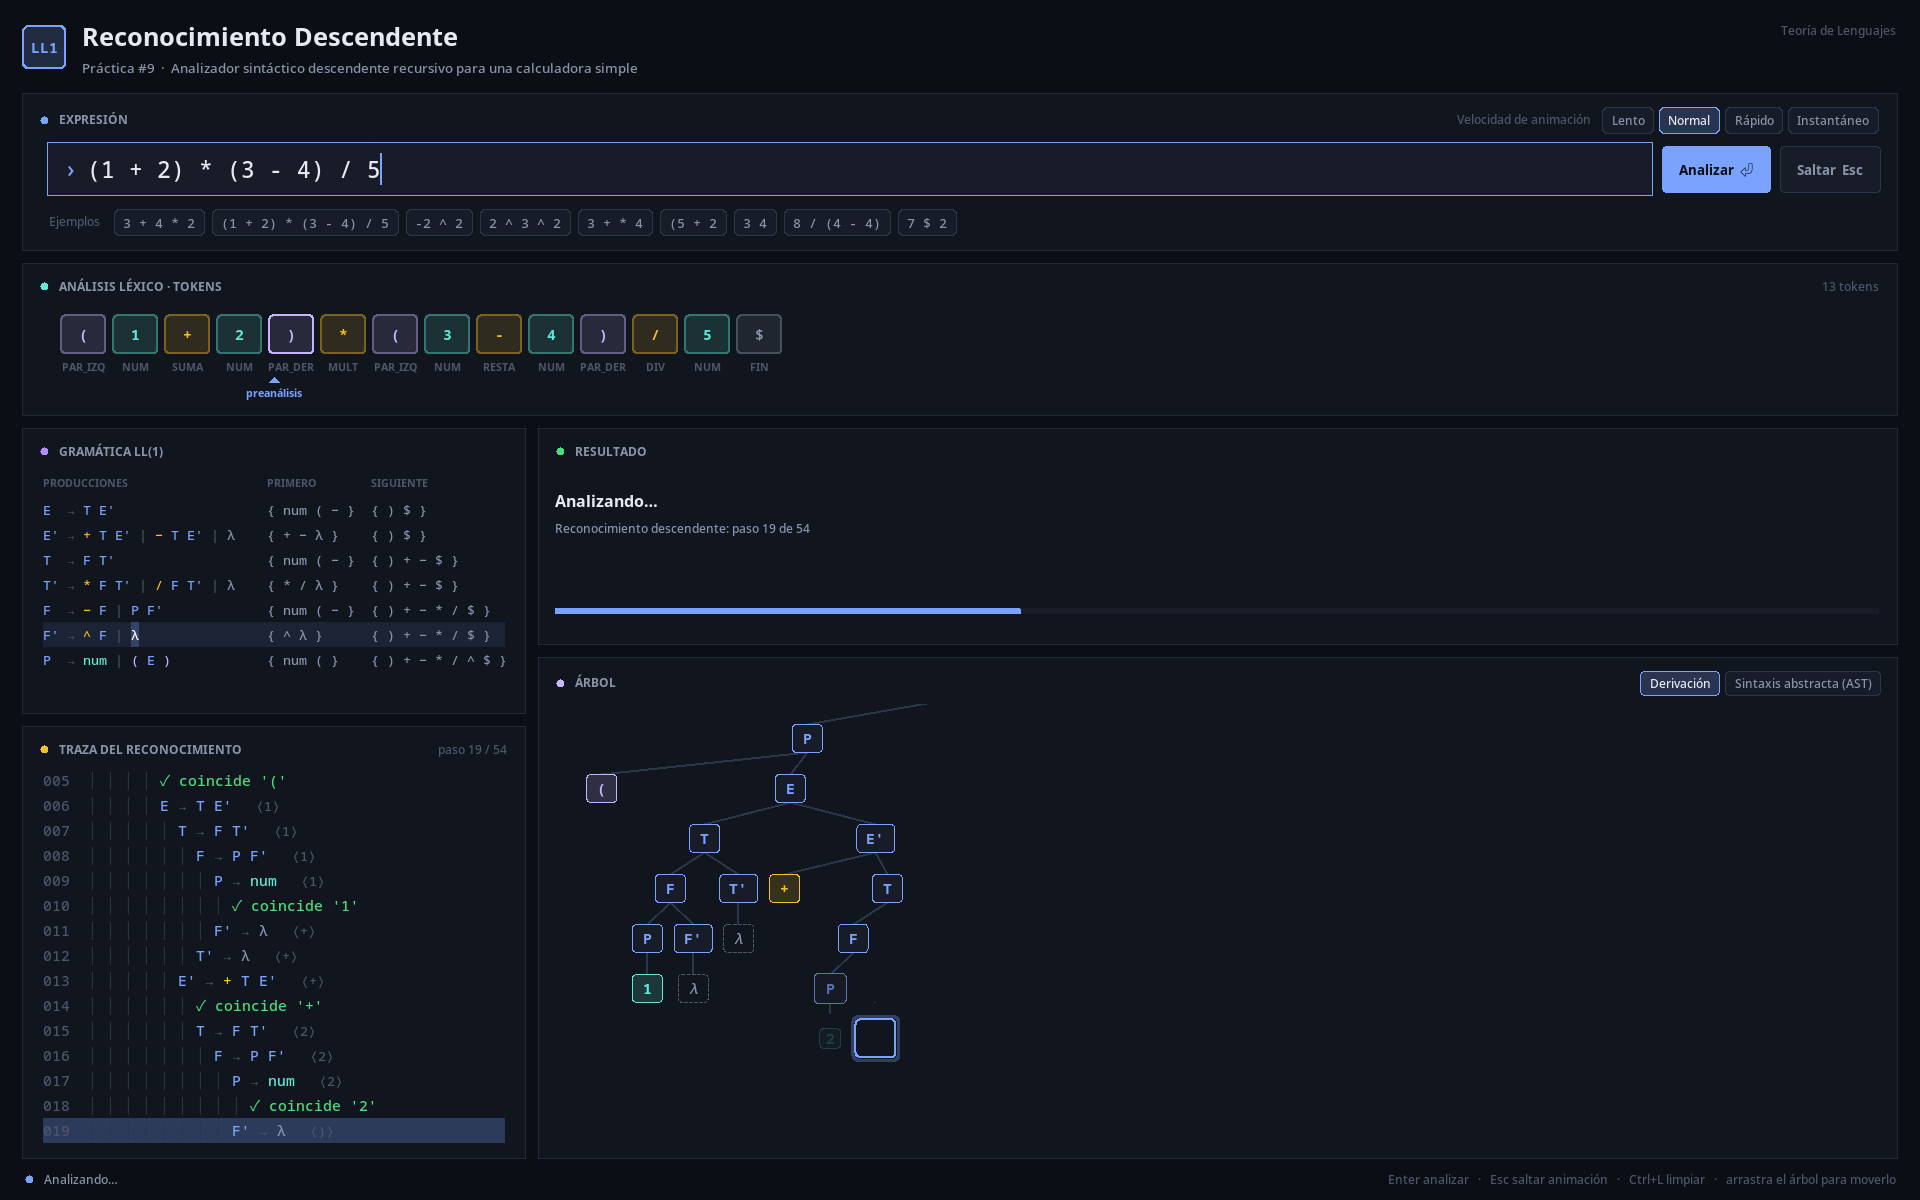
\includegraphics[width=\textwidth]{gui_animacion.png}
\caption{Interfaz durante el reconocimiento de \texttt{(1 + 2) * (3 - 4) / 5}, en el paso 19 de 54: el
puntero de preanálisis está sobre \tm{)}, la gramática resalta $\nt{F'}\to\lam$ y el árbol se está construyendo.}
\label{fig:gui}
\end{figure}

% ════════════════════════════════════════════════════════════════════════════
\section{Ejemplos desarrollados}

\subsection{Ejemplo 1: \texttt{3 + 4 * 2} (precedencia)}

\paragraph{Análisis léxico.}
\begin{center}
\begin{tikzpicture}[tok/.style={draw=#1, fill=#1!9, rounded corners=3pt, minimum width=10mm,
    minimum height=8mm, font=\ttfamily\bfseries, text=#1!85!black},
    lab/.style={font=\sffamily\tiny, text=gris}]
  \foreach \t/\c/\n [count=\i] in {3/numcolor/NUM, +/tmcolor/MAS, 4/numcolor/NUM, */tmcolor/POR, 2/numcolor/NUM, \$/gris/FIN}
  { \node[tok=\c] (t\i) at (\i*1.35,0) {\t}; \node[lab] at (\i*1.35,-0.7) {\n}; }
\end{tikzpicture}
\end{center}

\paragraph{Traza del reconocimiento.} La tabla~\ref{tab:traza1} es la salida del analizador: cada fila es
una expansión o un emparejamiento, sangrada según la profundidad de recursión. La columna de preanálisis
muestra el único token usado para decidir.

{\small
\begin{longtable}{r c L{6.6cm} c L{3.2cm}}
\caption{Traza del reconocimiento descendente de \texttt{3 + 4 * 2} (22 pasos).}\label{tab:traza1}\\
\toprule
\rowcolor{cabecera}\textbf{\#} & \textbf{Nivel} & \textbf{Acción} & \textbf{Preanálisis} & \textbf{Entrada restante} \\
\midrule\endfirsthead
\toprule
\rowcolor{cabecera}\textbf{\#} & \textbf{Nivel} & \textbf{Acción} & \textbf{Preanálisis} & \textbf{Entrada restante} \\
\midrule\endhead
\bottomrule\endfoot
\rowcolors{2}{white}{fila}
\gen{traza_ej1}
\end{longtable}}

\paragraph{Derivación por la izquierda.} Leyendo solo las expansiones de la traza se obtiene, en orden,
la derivación más a la izquierda de la cadena:

\begin{center}
\small\renewcommand{\arraystretch}{1.25}
\begin{tabular}{>{\color{gris}\scriptsize}r l @{\hspace{1.2cm}} >{\color{gris}\scriptsize}r l}
\toprule
\gen{derivacion_ej1}
\bottomrule
\end{tabular}
\end{center}
Al final, cada \tm{num} corresponde, en orden, a los lexemas \texttt{3}, \texttt{4} y \texttt{2}.

\paragraph{Árbol de derivación y AST.} El árbol de derivación (figura~\ref{fig:arbol1}) contiene todos
los símbolos de la gramática, incluidas las producciones vacías; el AST (figura~\ref{fig:ast1}) conserva
solo la estructura de operadores, y en él se ve que \tm{*} queda más profundo que \tm{+}: se evalúa primero.

\begin{figure}[H]
\centering
\gen{arbol_ej1}
\caption{Árbol de derivación de \texttt{3 + 4 * 2} generado por el analizador (\lam{} en líneas punteadas).}
\label{fig:arbol1}
\end{figure}

\begin{figure}[H]
\centering
\begin{minipage}{0.42\textwidth}\centering
\gen{ast_ej1}
\end{minipage}%
\begin{minipage}{0.4\textwidth}
\begin{tcolorbox}[colback=ok!4,colframe=ok!50,boxrule=0.5pt,arc=3pt,title={\sffamily\small Evaluación en postorden},
  colbacktitle=ok!15,coltitle=ok!30!black]
\gen{eval_ej1}
\end{tcolorbox}
\end{minipage}
\caption{AST de \texttt{3 + 4 * 2} anotado con el valor de cada subexpresión. Resultado: \textbf{11}.}
\label{fig:ast1}
\end{figure}

\begin{figure}[H]
\centering
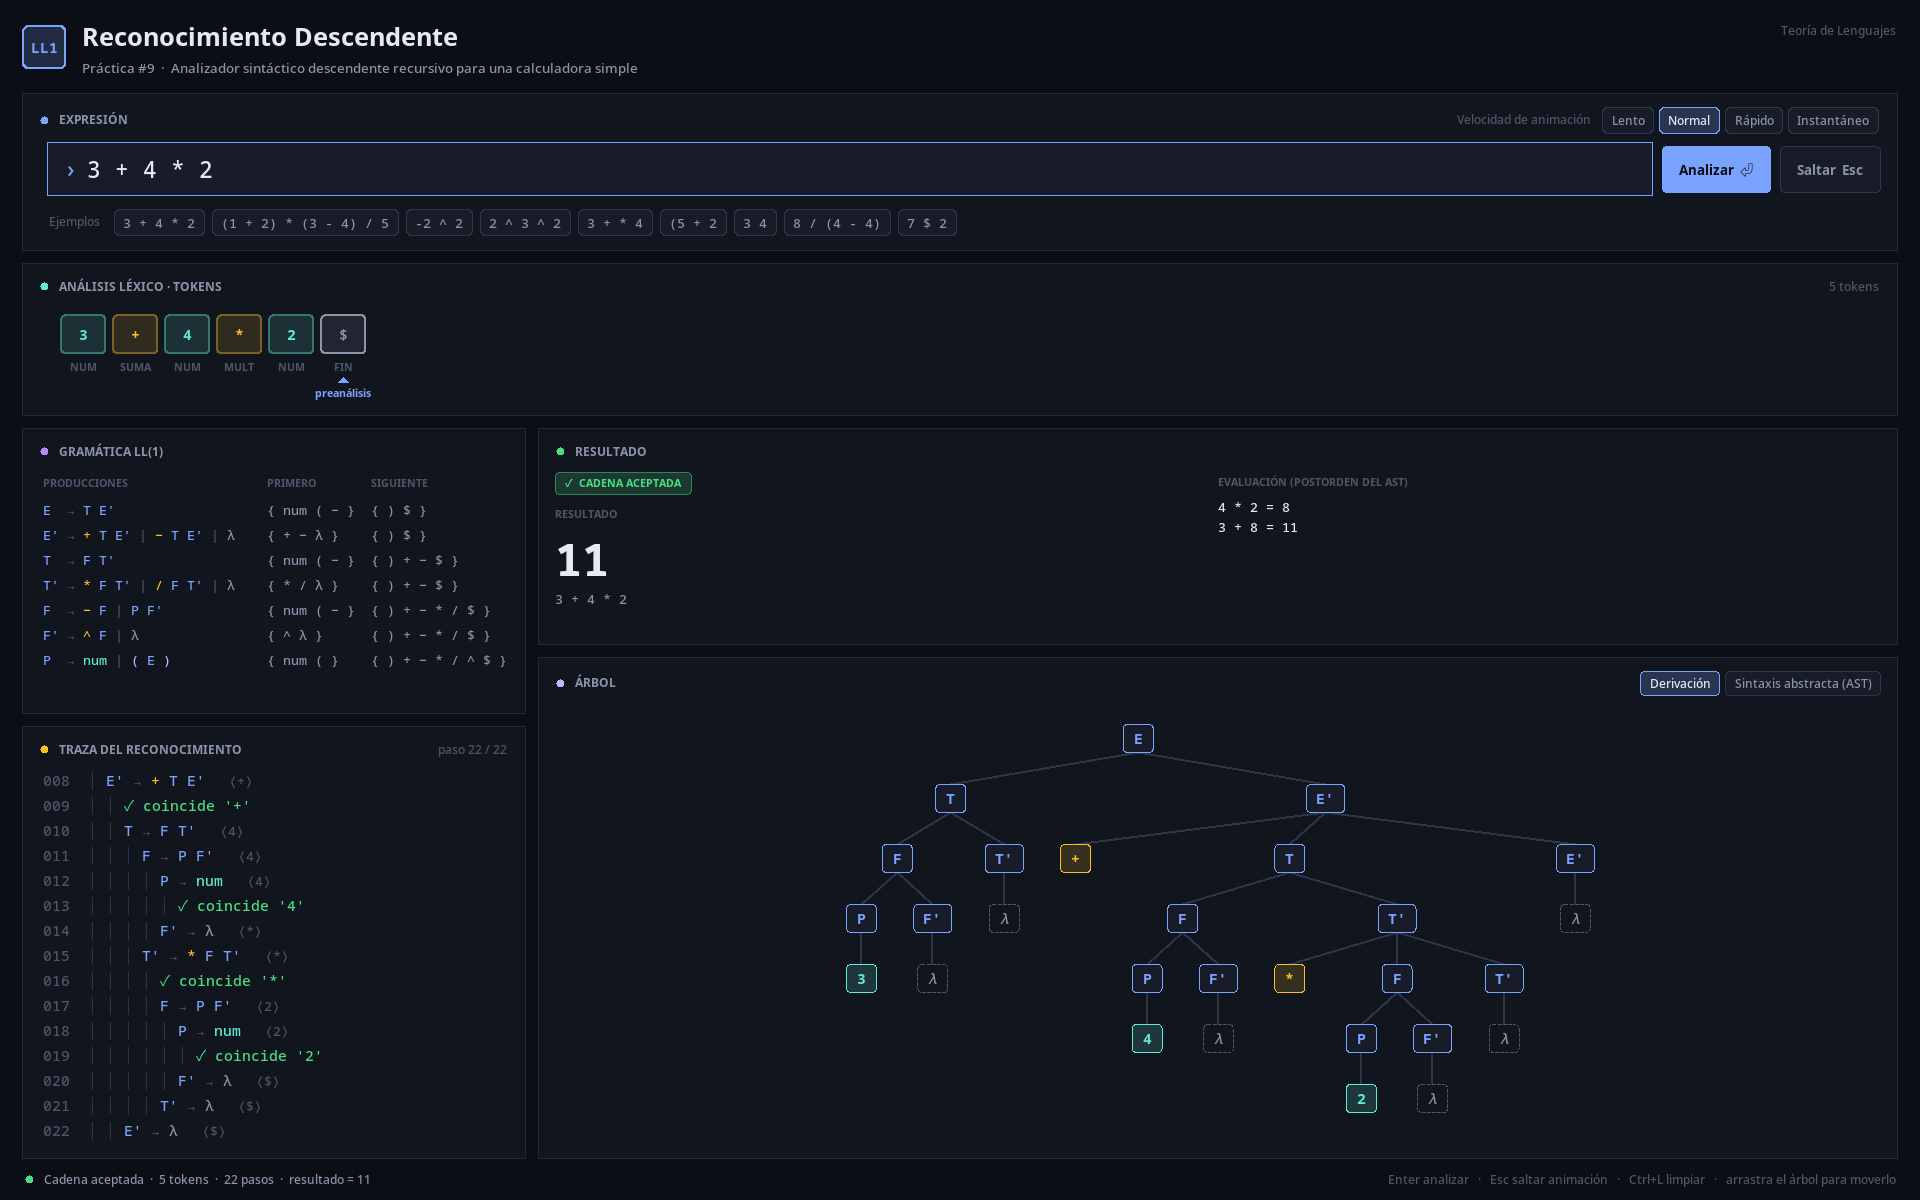
\includegraphics[width=\textwidth]{gui_aceptada.png}
\caption{Resultado en la interfaz: cadena aceptada, valor 11, pasos de evaluación y árbol de derivación completo.}
\end{figure}

\subsection{Ejemplo 2: asociatividad de la potencia y menos unario}

\begin{figure}[H]
\centering
\begin{subfigure}{0.32\textwidth}\centering
\gen{ast_pot}
\caption{\texttt{2 \^{} 3 \^{} 2} $=2^{(3^2)}=512$}
\end{subfigure}\hfill
\begin{subfigure}{0.3\textwidth}\centering
\gen{ast_neg}
\caption{\texttt{-2 \^{} 2} $=-(2^2)=-4$}
\end{subfigure}\hfill
\begin{subfigure}{0.34\textwidth}\centering
\scalebox{0.78}{\gen{arbol_pot}}
\caption{Derivación de \texttt{2 \^{} 3 \^{} 2}}
\end{subfigure}
\caption{La potencia anida hacia la derecha porque $\nt{F'}\to\tm{\^{}}\,\nt{F}$ reinicia el reconocimiento
de un factor completo; el menos unario queda por encima de \tm{\^{}} en el AST.}
\end{figure}

\subsection{Ejemplo 3: expresión compuesta}

Para \texttt{((2+3)*(4-1)\^{}2 - -8/2) * 3} el analizador realiza 84 pasos sobre 22 tokens.
El AST (figura~\ref{fig:largo}) muestra las ocho operaciones y sus valores intermedios.

\begin{figure}[H]
\centering
\begin{minipage}{0.55\textwidth}\centering
\gen{ast_largo}
\end{minipage}%
\begin{minipage}{0.4\textwidth}
\begin{tcolorbox}[colback=ok!4,colframe=ok!50,boxrule=0.5pt,arc=3pt,title={\sffamily\small Evaluación en postorden},
  colbacktitle=ok!15,coltitle=ok!30!black]
\gen{eval_largo}
\end{tcolorbox}
\end{minipage}
\caption{AST de \texttt{((2+3)*(4-1)\^{}2 - -8/2) * 3} $=147$.}
\label{fig:largo}
\end{figure}

\begin{figure}[H]
\centering
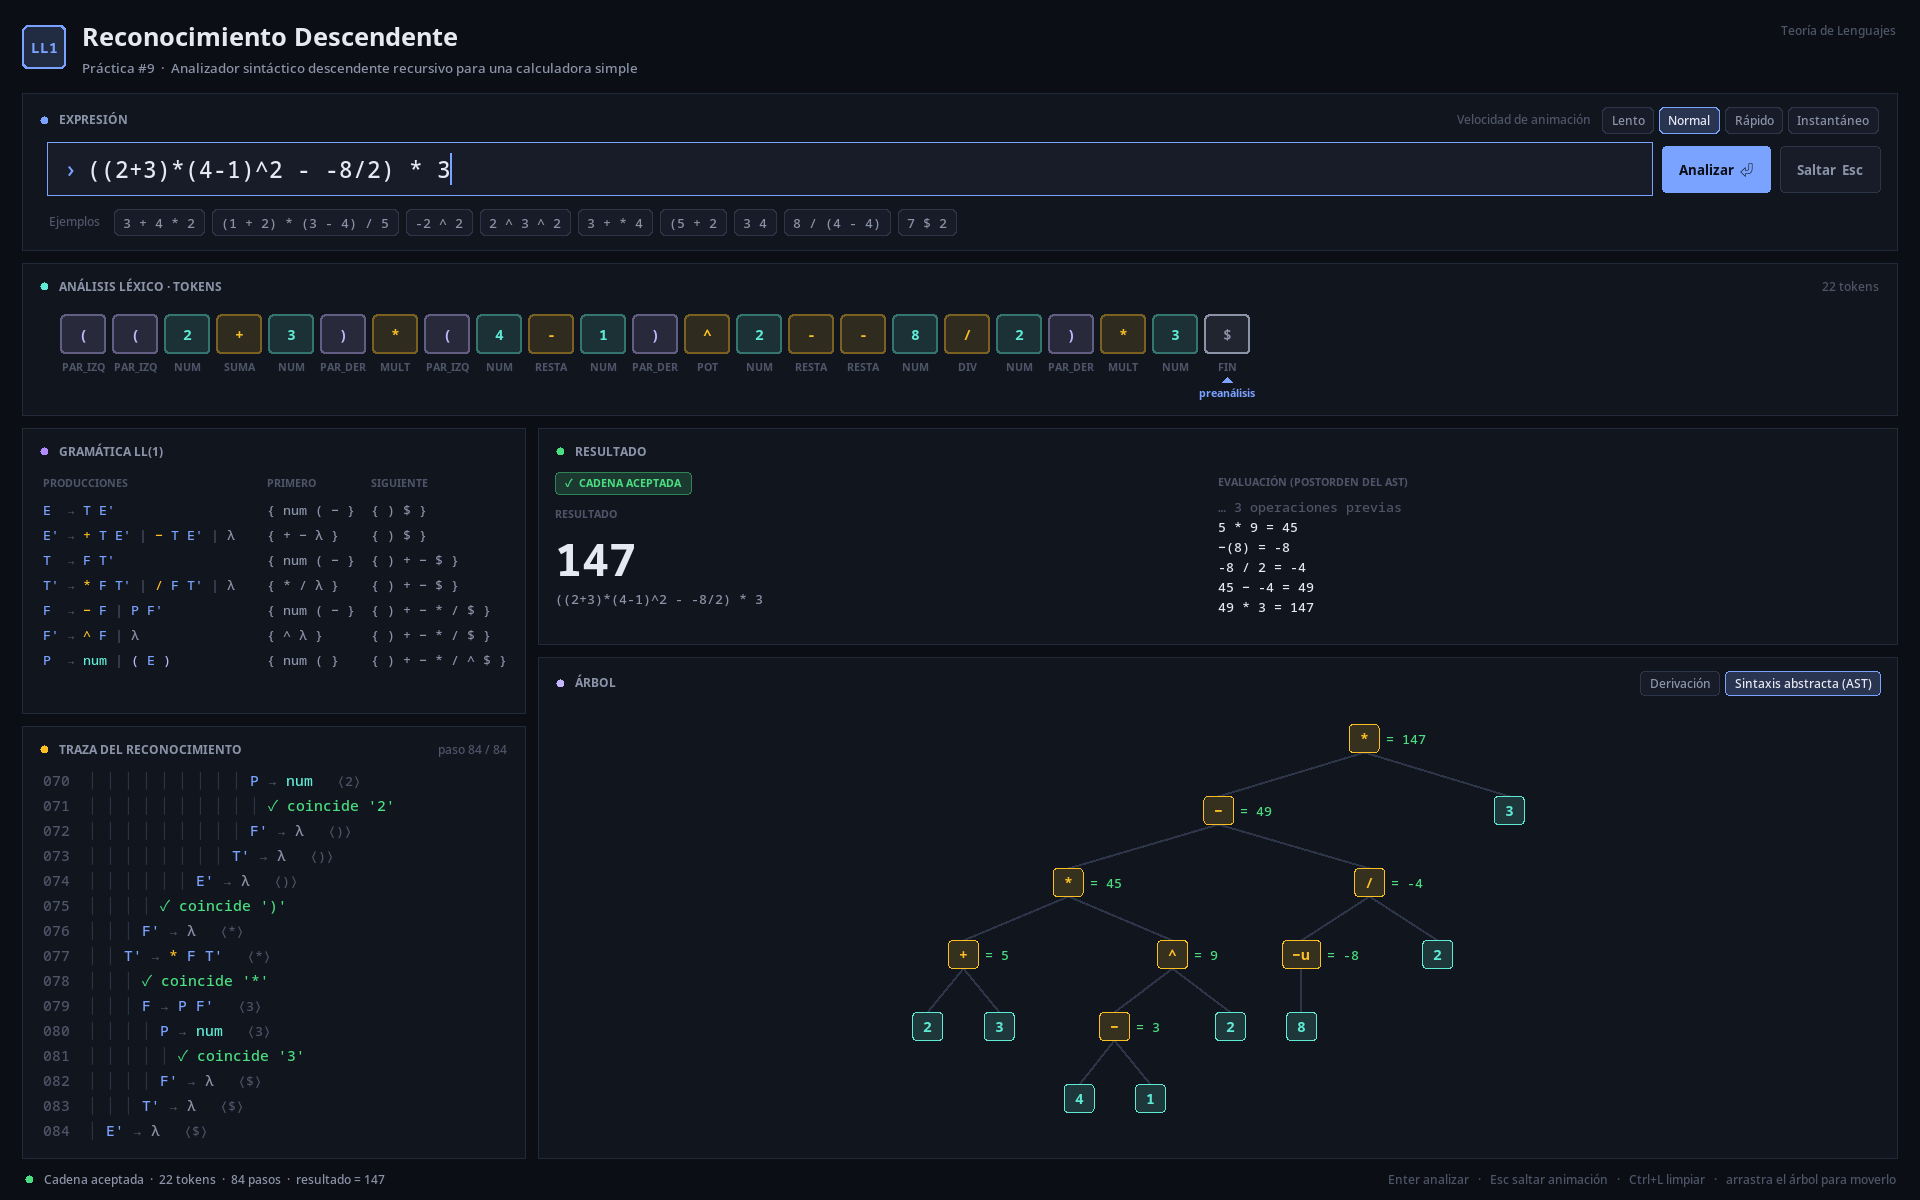
\includegraphics[width=\textwidth]{gui_ast.png}
\caption{Vista AST en la interfaz para la misma expresión.}
\end{figure}

\subsection{Ejemplo 4: error sintáctico \texttt{3 + * 4}}

Tras emparejar \tm{+}, $\nt{E'}$ llama a \texttt{T()}, éste a \texttt{F()} y éste a \texttt{P()}. El
preanálisis es \tm{*}, que no pertenece a $\PRIMERO(\nt{P})=\{\tm{num},\tm{(}\}$: falta un operando.
El error se detecta en el \emph{primer} token que no puede extender un prefijo válido, que es la
propiedad del prefijo viable de los analizadores \textsc{LL(1)}.

\begin{table}[H]
\centering
\caption{Traza de \texttt{3 + * 4}: el último paso es el diagnóstico.}
\small
\rowcolors{2}{white}{fila}
\begin{tabular}{r c L{8.6cm} c L{2cm}}
\toprule
\rowcolor{cabecera}\textbf{\#} & \textbf{Nivel} & \textbf{Acción} & \textbf{Preanálisis} & \textbf{Restante} \\
\midrule
\gen{traza_err}
\bottomrule
\end{tabular}
\end{table}

\begin{figure}[H]
\centering
\begin{minipage}{0.36\textwidth}\centering
\gen{arbol_err}
\end{minipage}\hfill
\begin{minipage}{0.6\textwidth}\centering
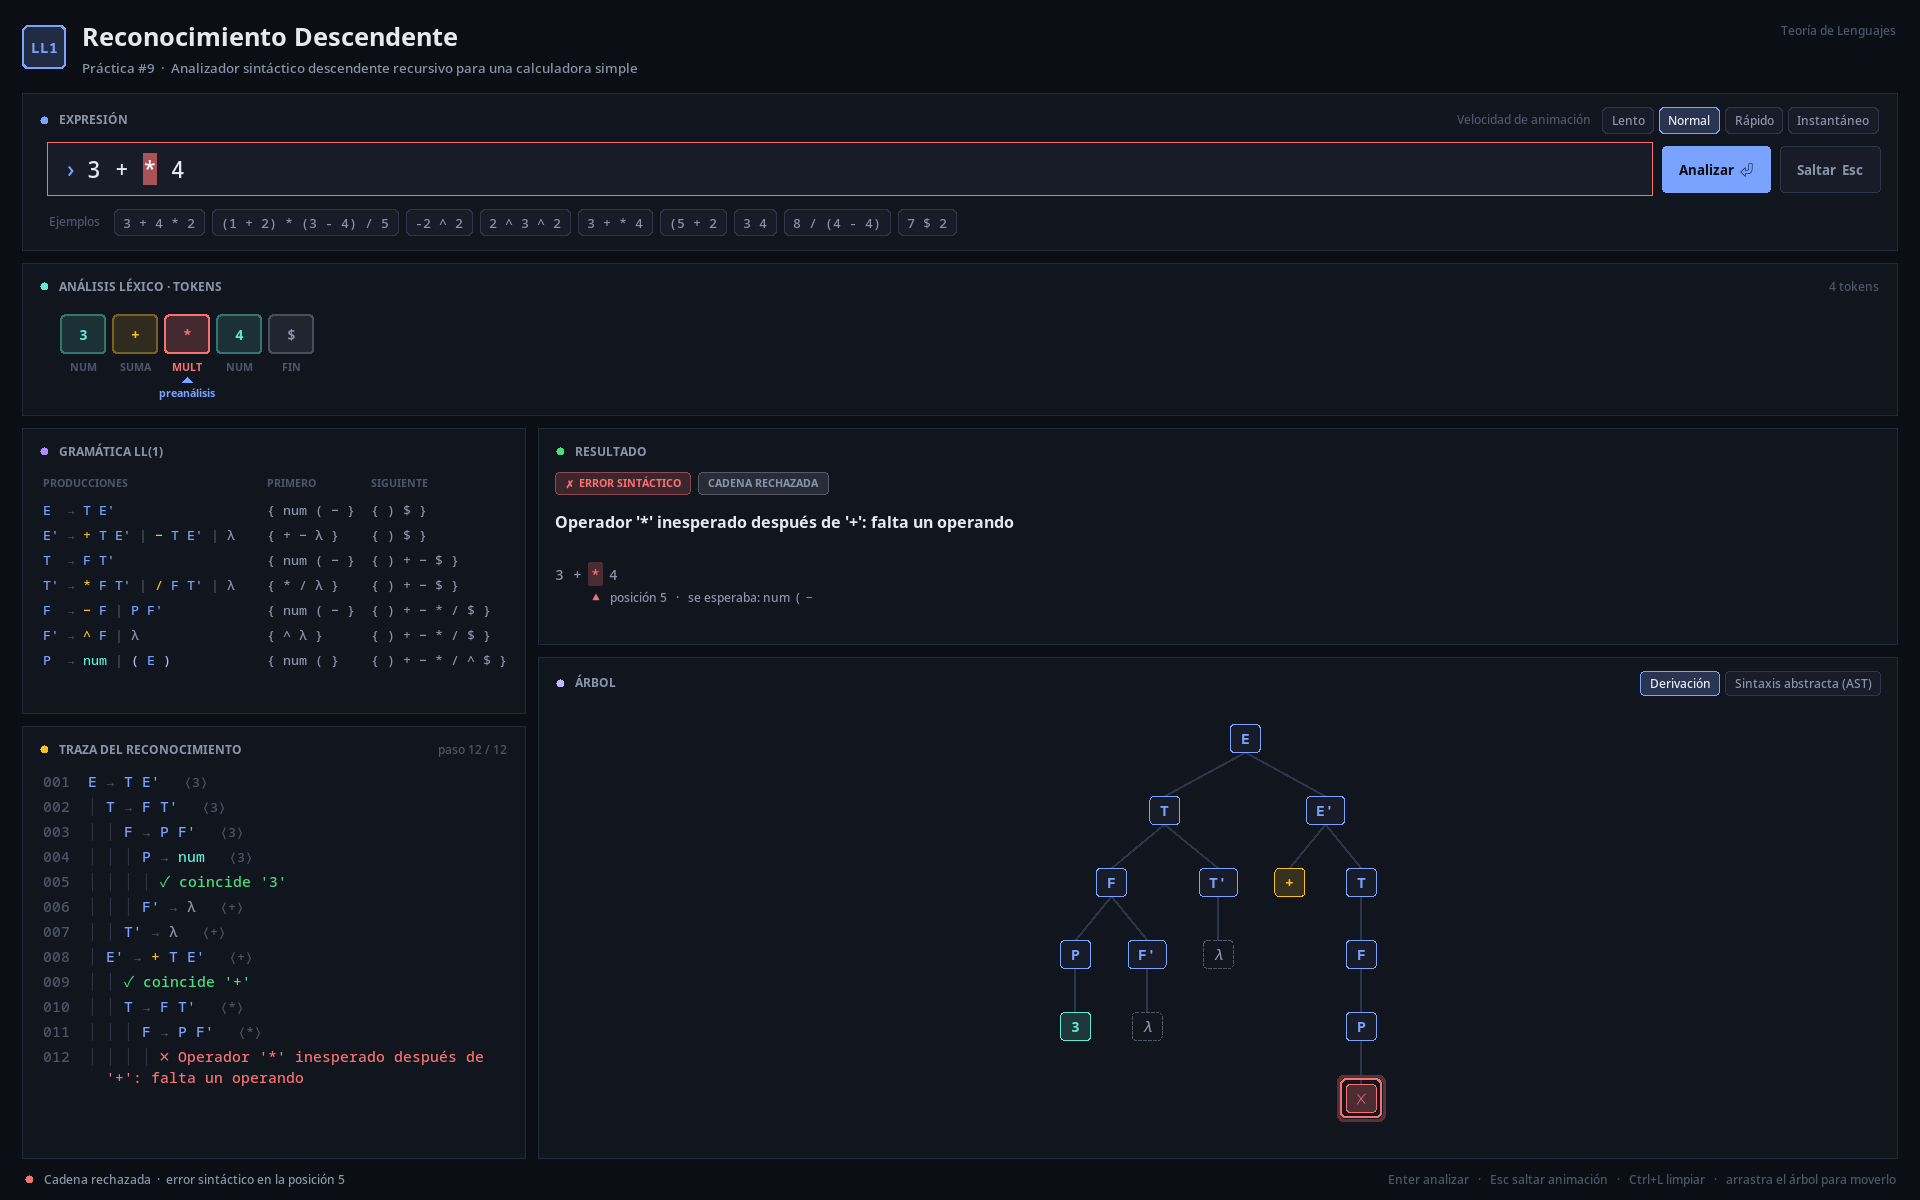
\includegraphics[width=\linewidth]{gui_error_sintactico.png}
\end{minipage}
\caption{Árbol parcial al momento del error (nodo \textcolor{err}{$\times$} bajo \nt{P}) y vista de la
interfaz: mensaje, posición 5, símbolos esperados (\tm{num}\;\tm{(}\;\tm{-}) y token marcado en rojo.}
\end{figure}

\subsection{Ejemplo 5: errores léxico y semántico}

\begin{figure}[H]
\centering
\begin{subfigure}{0.49\textwidth}
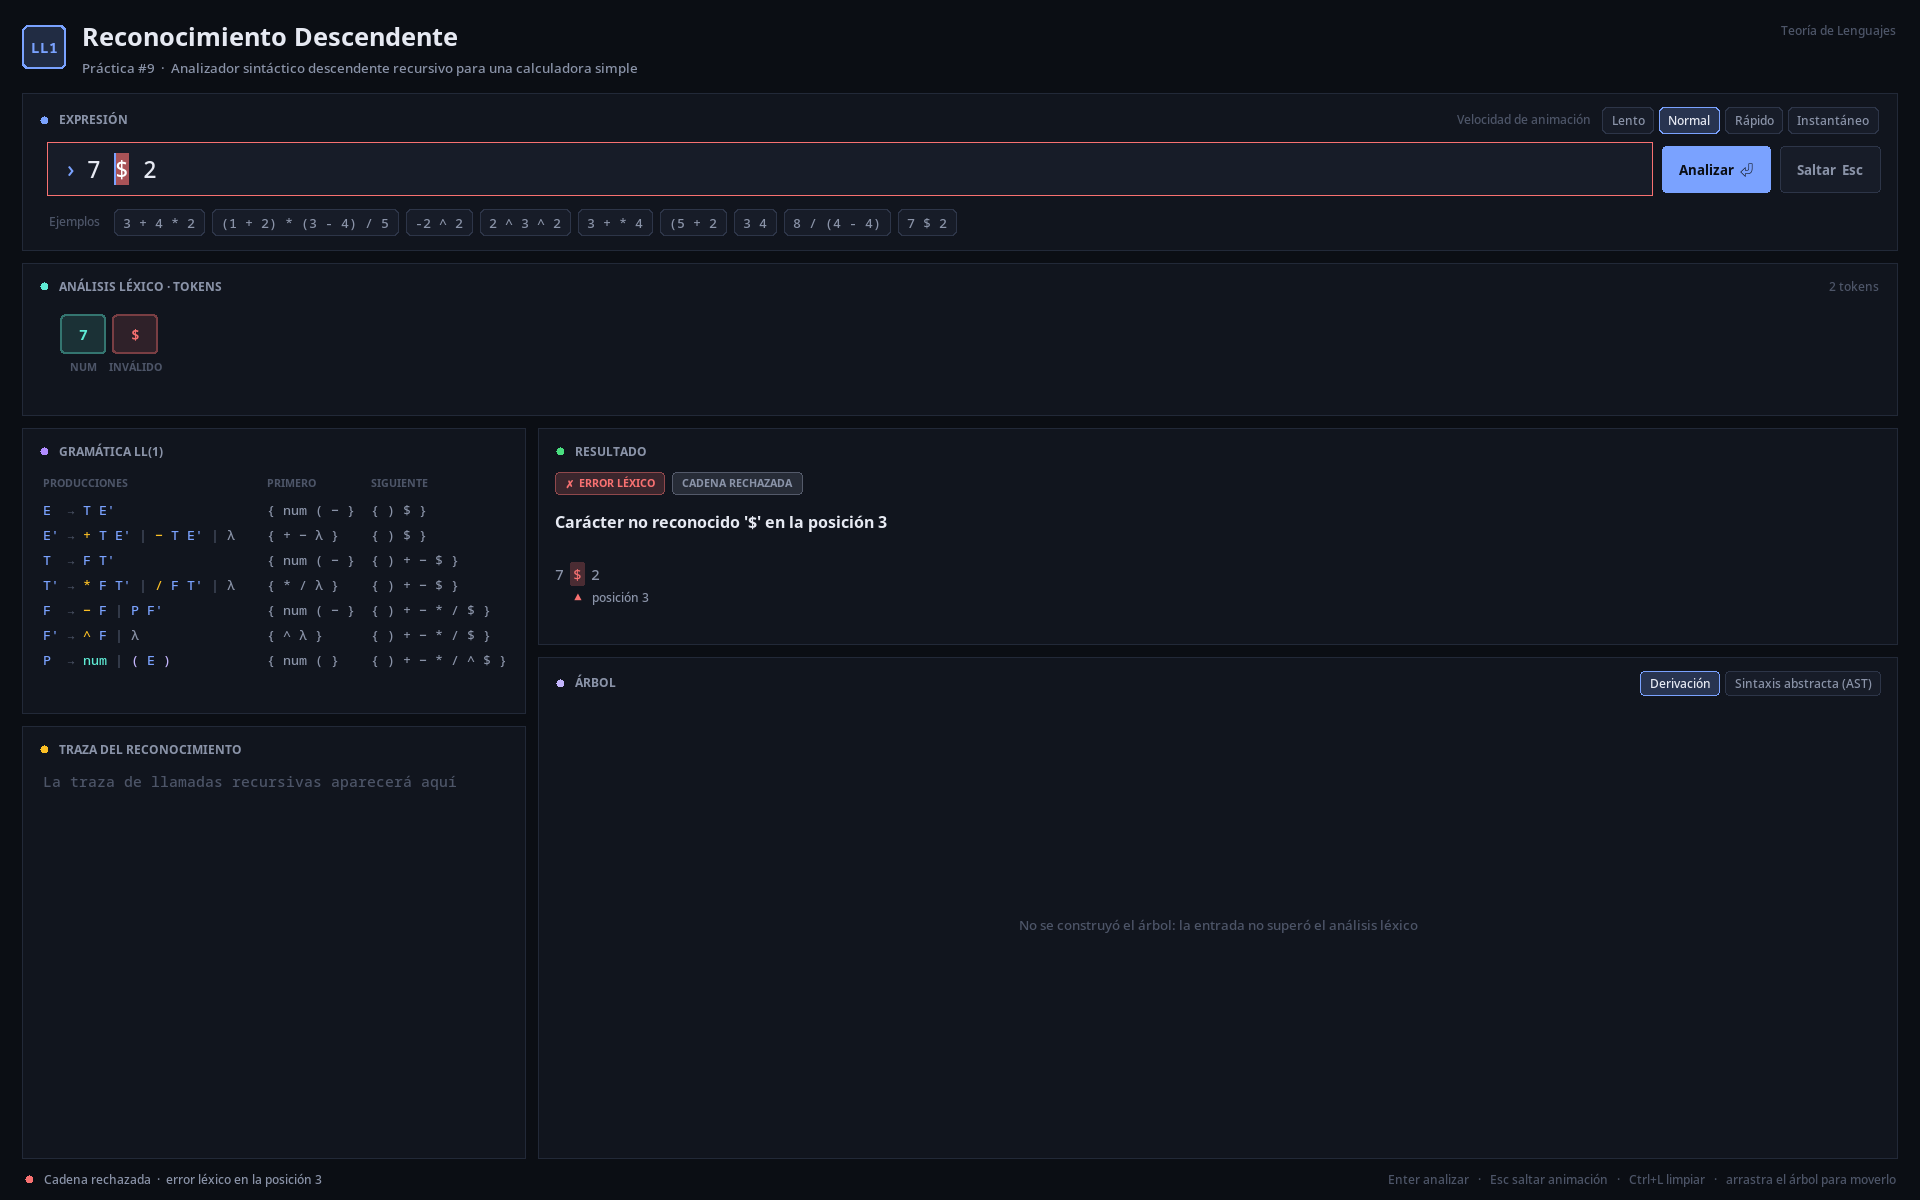
\includegraphics[width=\linewidth]{gui_error_lexico.png}
\caption{\texttt{7 \$ 2}: el símbolo \texttt{\$} no pertenece al alfabeto; no se inicia el análisis sintáctico.}
\end{subfigure}\hfill
\begin{subfigure}{0.49\textwidth}
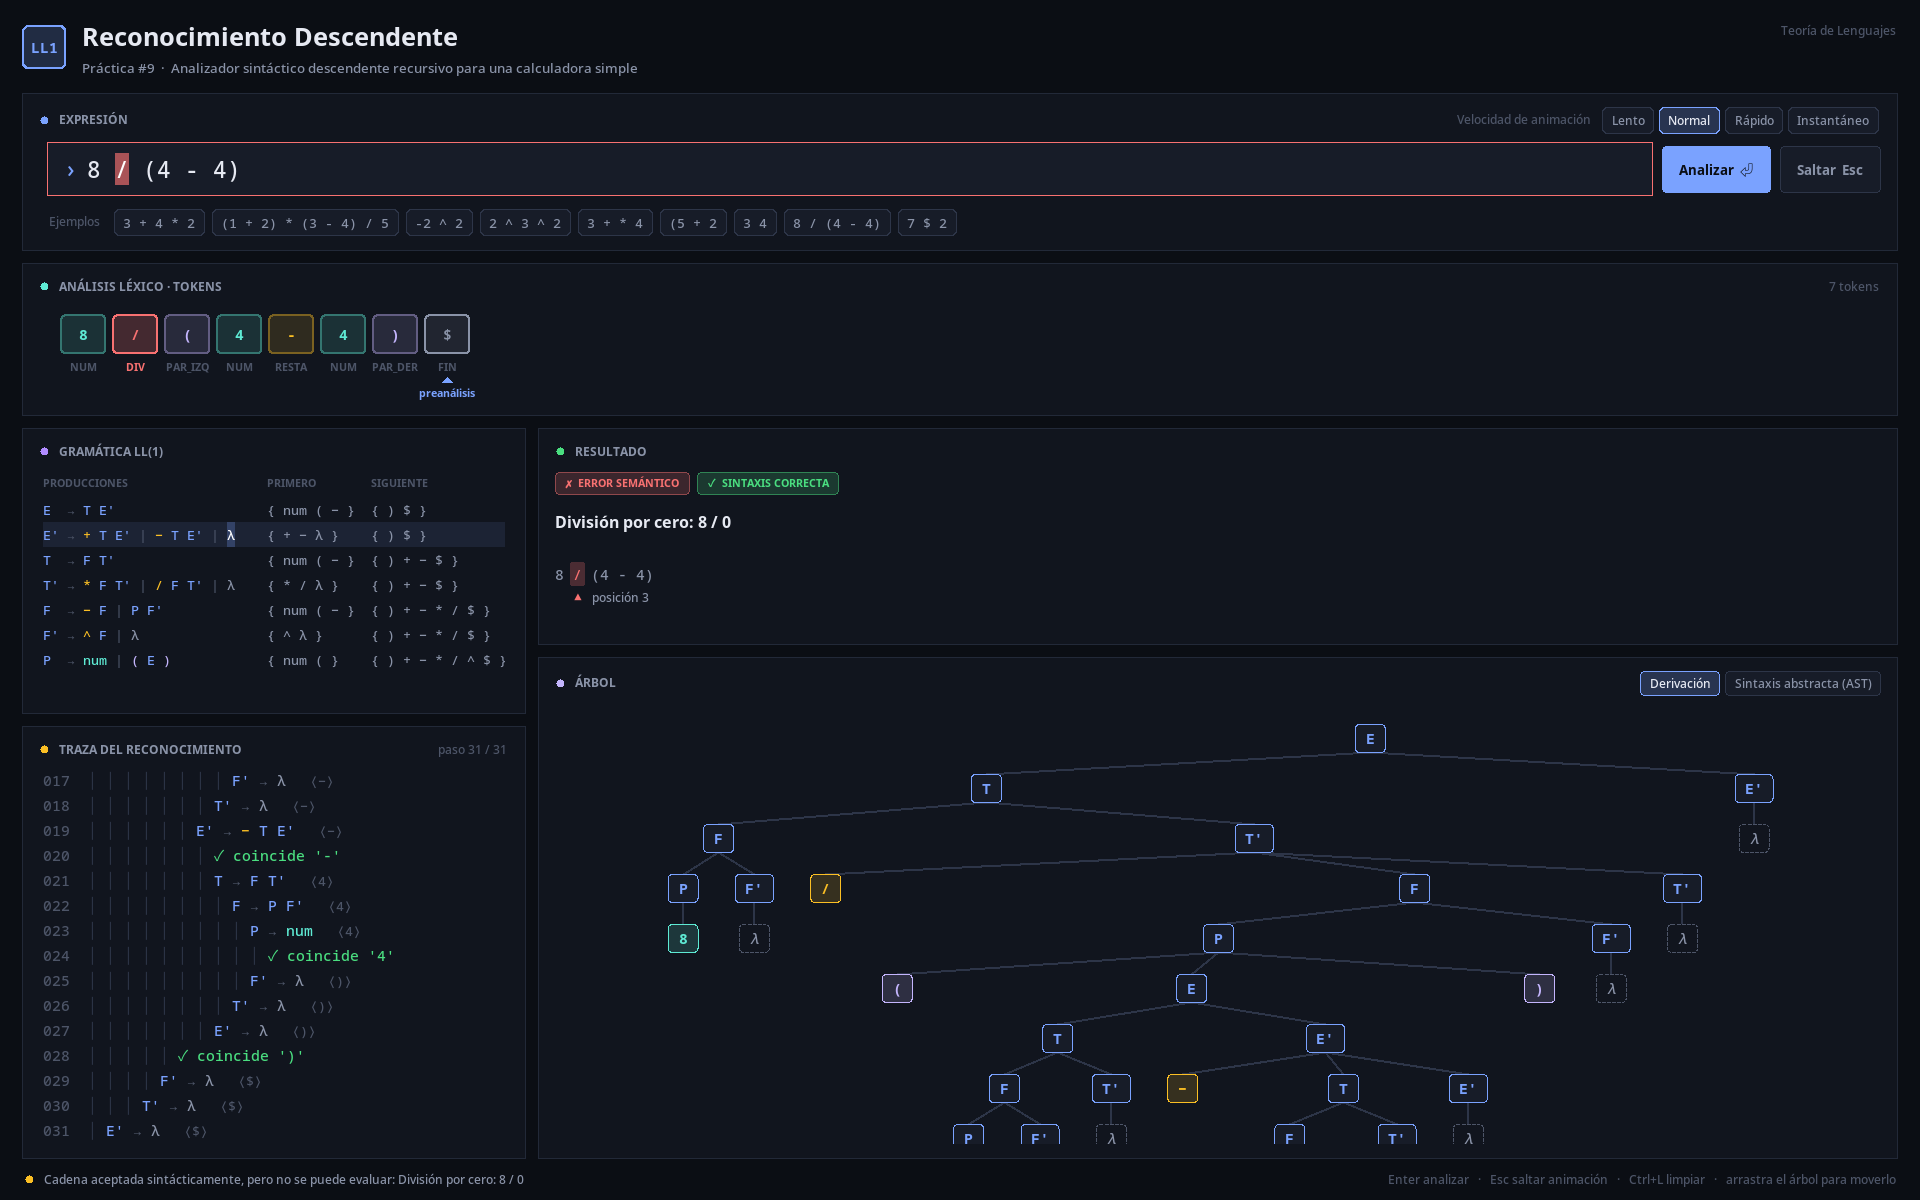
\includegraphics[width=\linewidth]{gui_error_semantico.png}
\caption{\texttt{8 / (4 - 4)}: sintaxis correcta, pero la división por cero impide evaluar.}
\end{subfigure}
\caption{Las tres clases de error se presentan con distinto distintivo; el error semántico aclara
que la cadena \emph{sí} pertenece al lenguaje.}
\end{figure}

% ════════════════════════════════════════════════════════════════════════════
\section{Pruebas y resultados}

\subsection{Batería de pruebas}

La tabla~\ref{tab:pruebas} se genera ejecutando el analizador sobre 26 entradas que cubren precedencia,
asociatividad, menos unario, decimales, anidamiento, los símbolos alternativos y todos los tipos de
error. En todos los casos el comportamiento obtenido coincide con el esperado.

{\small
\rowcolors{2}{white}{fila}
\begin{longtable}{r L{3.3cm} L{3.3cm} c L{5.2cm}}
\caption{Resultados de la batería de pruebas (salida real del programa).}\label{tab:pruebas}\\
\toprule
\rowcolor{cabecera}\textbf{\#} & \textbf{Entrada} & \textbf{Propósito} & \textbf{Veredicto} & \textbf{Resultado o mensaje} \\
\midrule\endfirsthead
\toprule
\rowcolor{cabecera}\textbf{\#} & \textbf{Entrada} & \textbf{Propósito} & \textbf{Veredicto} & \textbf{Resultado o mensaje} \\
\midrule\endhead
\bottomrule\endfoot
\gen{pruebas}
\end{longtable}}

\subsection{Costo del reconocimiento}

Cada token se empareja exactamente una vez y entre dos emparejamientos solo hay un número acotado de
expansiones (a lo sumo la cadena $\nt{E}\to\nt{T}\to\nt{F}\to\nt{P}$ y los cierres \lam{}), por lo que
el número de pasos crece \emph{linealmente} con el número de tokens: el analizador es $O(n)$ en tiempo y,
por la pila de recursión, $O(d)$ en memoria, con $d$ la profundidad de anidamiento. La figura~\ref{fig:costo}
lo confirma empíricamente sobre 140 expresiones válidas generadas al azar.

\begin{figure}[H]
\centering
\begin{tikzpicture}
\begin{axis}[
  width=0.82\textwidth, height=6.4cm,
  xlabel={\sffamily\small tokens de entrada $n$}, ylabel={\sffamily\small cantidad},
  grid=major, grid style={draw=gris!15}, axis line style={draw=gris!50},
  tick label style={font=\sffamily\scriptsize}, legend pos=north west,
  legend style={font=\sffamily\scriptsize, draw=gris!30, fill=white, fill opacity=0.9, text opacity=1},
  xmin=0, ymin=0]
\addplot[only marks, mark=*, mark size=1.5pt, color=acento, fill opacity=0.55, draw opacity=0.7]
  table[x=tokens, y=pasos] {gen/complejidad.dat};
\addlegendentry{pasos del reconocimiento}
\addplot[only marks, mark=square*, mark size=1.3pt, color=parcolor, fill opacity=0.45, draw opacity=0.6]
  table[x=tokens, y=nodos] {gen/complejidad.dat};
\addlegendentry{nodos del árbol de derivación}
\addplot[thick, color=acento!70!black, no marks]
  table[x=tokens, y={create col/linear regression={y=pasos}}] {gen/complejidad.dat};
\addlegendentry{ajuste lineal: $\approx\pgfmathprintnumber[precision=2]{\pgfplotstableregressiona}\,n
  \pgfmathprintnumber[precision=1,showpos]{\pgfplotstableregressionb}$}
\end{axis}
\end{tikzpicture}
\caption{Pasos del analizador y tamaño del árbol de derivación frente al número de tokens: ambos siguen
una recta, confirmando el costo lineal del análisis \textsc{LL(1)}.}
\label{fig:costo}
\end{figure}

% ════════════════════════════════════════════════════════════════════════════
\section{Manual de uso}

\textbf{Requisitos.} Python 3.10 o superior con \texttt{tkinter} (incluido en las instalaciones estándar
de Windows y macOS; en Linux, paquete \texttt{python3-tk} o \texttt{tk}). No hay dependencias externas.

\begin{tcolorbox}[colback=tinta,colframe=tinta,coltext=white,arc=3pt,left=10pt,boxrule=0pt]
\ttfamily\small
\textcolor{gris!60}{\# interfaz gráfica}\\
\$ python3 app.py\\[4pt]
\textcolor{gris!60}{\# modo consola: tokens, traza, evaluación y resultado}\\
\$ python3 analizador.py "3 + 4 * 2"\\[4pt]
\textcolor{gris!60}{\# regenerar tablas, trazas y árboles de este informe}\\
\$ cd informe \&\& python3 generar.py \&\& pdflatex informe.tex
\end{tcolorbox}

\begin{table}[H]
\centering
\caption{Controles de la interfaz gráfica.}
\begin{tabular}{l L{10.5cm}}
\toprule
\rowcolor{cabecera}\textbf{Control} & \textbf{Acción} \\
\midrule
\texttt{Enter} / \textsf{Analizar} & Analiza la expresión escrita y anima el reconocimiento. \\
\texttt{Esc} / \textsf{Saltar}     & Completa la animación en curso de inmediato. \\
\texttt{Ctrl+L}                    & Limpia la entrada y todos los paneles. \\
\textsf{Ejemplos}                  & Nueve expresiones de un clic, válidas e inválidas. \\
\textsf{Velocidad}                 & Lento, Normal, Rápido o Instantáneo (cambiable durante la animación). \\
\textsf{Derivación / AST}          & Alterna entre el árbol de derivación y el árbol de sintaxis abstracta. \\
Arrastrar / rueda                  & Desplaza el árbol cuando no cabe en el panel. \\
\bottomrule
\end{tabular}
\end{table}

% ════════════════════════════════════════════════════════════════════════════
\section{Conclusiones}

\begin{itemize}[label=\textcolor{acento}{$\blacktriangleright$}]
\item La gramática natural de una calculadora es ambigua; estratificarla por precedencia, eliminar la
      recursividad por la izquierda y factorizarla produce una gramática \textsc{LL(1)} equivalente, cuya
      tabla de análisis se verificó automáticamente sin conflictos.
\item El descenso recursivo traduce esa gramática a código de manera casi mecánica ---un procedimiento por
      no terminal--- y su traza coincide paso a paso con la derivación por la izquierda de la cadena.
\item La recursividad por la derecha introducida por la transformación no altera la semántica: un atributo
      heredado permite construir un AST con la asociatividad izquierda correcta, mientras que la potencia
      conserva su asociatividad derecha.
\item Elegir \lam{} únicamente cuando el preanálisis está en \SIGUIENTE{} hace que los errores se reporten en
      el primer token inválido, con mensajes precisos y la lista de símbolos esperados.
\item Separar errores léxicos, sintácticos y semánticos aclara al usuario si su cadena pertenece o no al
      lenguaje, aun cuando no pueda evaluarse.
\item El análisis es lineal en el tamaño de la entrada, como se comprobó experimentalmente; y la
      visualización animada convierte un proceso abstracto en uno observable, útil como herramienta didáctica.
\end{itemize}

% ════════════════════════════════════════════════════════════════════════════
\section*{Referencias}
\addcontentsline{toc}{section}{Referencias}
\begin{enumerate}[label={[\arabic*]}, leftmargin=*, itemsep=4pt]
\item A.~V. Aho, M.~S. Lam, R.~Sethi y J.~D. Ullman. \emph{Compiladores: principios, técnicas y herramientas},
      2.ª ed. Pearson, 2008. Cap.~4: Análisis sintáctico.
\item J.~E. Hopcroft, R.~Motwani y J.~D. Ullman. \emph{Introducción a la teoría de autómatas, lenguajes y
      computación}, 3.ª ed. Pearson, 2007.
\item K.~D. Cooper y L.~Torczon. \emph{Engineering a Compiler}, 2nd ed. Morgan Kaufmann, 2011. Cap.~3.
\item N.~Wirth. \emph{Compiler Construction}. Addison-Wesley, 1996. Cap.~4: Análisis descendente recursivo.
\item Python Software Foundation. \emph{tkinter --- Python interface to Tcl/Tk}.
      \url{https://docs.python.org/3/library/tkinter.html}
\end{enumerate}

% ════════════════════════════════════════════════════════════════════════════
\appendix
\section{Cálculo de PRIMERO y SIGUIENTE}

\codigo{analizador.py — calcular\_primero\_siguiente()}{gen/codigo_conjuntos.py}

\end{document}
